%!TEX program = xelatex

\documentclass[12pt, a4paper]{report}
\usepackage[legalpaper, a4paper, margin=2cm]{geometry}
\usepackage[french]{babel}
\usepackage{hyperref}
\usepackage{libs/utbmcovers}
\usepackage{lipsum}
\usepackage{sectsty}
\usepackage{csquotes}
% \documentclass{article}
\usepackage{float}
\usepackage{graphicx} % Requis pour insérer des images
\usepackage{svg}
\usepackage{tikz}


\usepackage[
	backend=biber,
	style=authortitle,
	citestyle=verbose-ibid,
	abbreviate=false,
	language=french,
	datamodel=ISO690UTBM
]{biblatex} % ISO 690 Utbm

\input{biblatex.cfg}

%----------------------------------------
% Use Arial as base font
%----------------------------------------

\setmainfont{Arial.ttf}[
	Path=./assets/fonts/, 
	Extension=.ttf, 
	BoldFont = *Bold, 
	ItalicFont = *Italic, 
	BoldItalicFont = *BoldItalic,
]

\chapterfont{\arialfont\fontseries{b}\fontsize{28pt}{36pt}}
\sectionfont{\arialfont\fontseries{b}\fontsize{24pt}{28pt}}
\subsectionfont{\arialfont\fontseries{b}\fontsize{20pt}{22pt}}
\subsubsectionfont{\arialfont\fontseries{b}\fontsize{20pt}{22pt}}

%----------------------------------------
% UTBM covers configuration
%----------------------------------------

% \setutbmfrontillustration{}
\setutbmtitle{Analyse de la consommation énergétique du DNS}
\setutbmsubtitle{Rapport de stage ST50 - P2026}
\setutbmstudent{LEROY Fernand}
\setutbmstudentdepartment{FISE-INFO}
\setutbmstudentpathway{Data Science et IA}
\setutbmcompany{Télécom SudParis}
\setutbmcompanyaddress{19 Place Marguerite Perey \\ 91120 Palaiseau}
\setutbmcompanywebsite{www.telecom-sudparis.eu}
\setutbmcompanytutor{MAROT Michel}
\setutbmschooltutor{BAALA CANALDA Oumaya}
% \setutbmabstract{}

%----------------------------------------
% Document configuration
% Notes:
% - '\graphicspath' refers to the path where images are stored.
% - '\addbibresource' refers to the bibliography file(s), separated by commas.
%----------------------------------------

\graphicspath{{./assets/images/}}
\addbibresource{bibliography.bib}
\usetikzlibrary{arrows.meta, fit, backgrounds}
\graphicspath{ {/Graphs} }

%----------------------------------------
% Document
% Notes:
% - Usually, the abstract is not referenced in the table of contents
%	  nor the greetings section, so we use the '*' option to avoid it.
% - Non-cited references are not shown in the bibliography, so we use the
%	  '\nocite{*}' command to show them.
% - Everything below '\subsubsection' is not shown in the table of contents,
%----------------------------------------

\begin{document}
	\arialfont

	\makeutbmfrontcover{}
 
	\section*{Abstract}
	\lipsum[1-3]
	
	\newpage

	\section*{Remerciements}
	\lipsum[1-2] 

	\tableofcontents
	\newpage

	\chapter*{Introduction}
	\addcontentsline{toc}{chapter}{Introduction}

	\textbf{Contexte :} \\
	Les DNS sont utilisés quotidiennement.
	\textbf{Problème :} \\
	Nous devons trouver une méthode pour mesurer et estimer la consommation énergétique du DNS, incluant tous les acteurs différents présents dans le processus de résolution d'un nom de domaine. Mesurer un système distribué comme le DNS n'est pas simple et implique l'estimation de la consommation énergétique de tous les acteurs du système. Pour simplifier le problème, nous nous sommes d'abord concentrés sur l'estimation de la consommation énergétique du premier acteur : le résolveur.

	\textbf{Travaux connexes :}
	Ce document s'appuie sur les travaux d'anciens stagiaires ayant mesuré la même configuration : *Analyse de la consommation énergétique des résolveurs DNS* \cite{ResolverEnergy}.

	\textbf{Défis ou lacunes :}
	Les études précédentes sur la consommation énergétique des résolveurs DNS manquent d'interprétabilité. Celle-ci est importante pour modéliser cette consommation et estimer la consommation énergétique de différents types de résolveurs à différentes échelles. De plus, contrairement à d'autres études, la méthode utilisée pour mesurer la consommation énergétique du cache du résolveur utilise le même ensemble de domaines que celui utilisé pour mesurer le résolveur sans cache. \textbf{Cela permet une estimation de la consommation énergétique plus proche des cas d'usage réels}. Pour l'estimation de la consommation énergétique de la résolution sans utilisation du cache, la configuration est modifiée pour empêcher la mise en cache des domaines qui pourraient réapparaître et fausser les résultats.

	\textbf{Idée principale :}
	Comparaison de deux approches pour modéliser la consommation énergétique de Bind9, une implémentation de résolveur DNS. La première consiste à analyser son fonctionnement pour créer un modèle de file d'attente qui nous aidera à estimer la consommation énergétique. La deuxième approche est agnostique : la complexité algorithmique du logiciel est analysée temporellement et spatialement, de manière statique et pendant l'exécution.
	// Il faudrait une petite comparaison entre les deux approches pour expliquer leurs différences et limitations.

	\textbf{Contributions :}
	\begin{itemize}
		\item Méthode d'estimation de la consommation énergétique des logiciels/DNS
		\item Étude de la consommation via un modèle de file d'attente
		\item Étude de la consommation via une analyse du code d'une implémentation DNS (Bind9)
	\end{itemize}

	\textbf{Organisation :} du document / rapport

	---
	\chapter{Présentation de Télécom SudParis}

	\section{Présentation de l'organisme d'accueil}

	\subsection{Télécom SudParis dans son environnement international, européen et français}

	Télécom SudParis est une grande école d'ingénieurs française spécialisée dans les technologies du numérique, les télécommunications, les réseaux, l'informatique et la cybersécurité. Depuis 2019, elle est membre de l'Institut Polytechnique de Paris (IP Paris), qui rassemble plusieurs grandes écoles françaises de premier plan telles que l'École Polytechnique, Télécom Paris, l'ENSTA Paris et l'ENSAE Paris. Cette intégration lui permet de bénéficier d'une forte visibilité académique et scientifique à l'échelle internationale.

	Au niveau européen, Télécom SudParis participe à de nombreux projets de recherche et collabore avec des universités, laboratoires et entreprises du secteur numérique. Ses activités de recherche couvrent notamment les réseaux de communication, la cybersécurité, l'intelligence artificielle et les systèmes distribués.

	Au niveau national, l'école appartient également à l'Institut Mines-Télécom (IMT), premier groupe public français d'écoles d'ingénieurs et de management dédié à la transformation numérique, industrielle et énergétique. Télécom SudParis contribue ainsi à la formation d'ingénieurs et de chercheurs capables de répondre aux enjeux technologiques actuels et futurs.

	\subsection{Télécom SudParis au sein de l'Institut Mines-Télécom et de l'Institut Polytechnique de Paris}

	Fondée en 1979 sous le nom d'Institut National des Télécommunications (INT), Télécom SudParis est aujourd'hui l'une des écoles de l'Institut Mines-Télécom tout en étant membre de l'Institut Polytechnique de Paris. Elle a pour mission de former des ingénieurs, chercheurs et experts du numérique grâce à un enseignement de haut niveau associé à une activité de recherche reconnue.

	L'école est organisée autour de plusieurs départements d'enseignement et de recherche couvrant différents domaines du numérique, tels que les réseaux, l'informatique, les systèmes embarqués ou encore la cybersécurité. Elle entretient de nombreux partenariats avec des acteurs industriels et académiques, en France comme à l'étranger.

	Durant mon stage, j'ai été accueilli sur le campus de Palaiseau, situé au sein du cluster scientifique de l'Institut Polytechnique de Paris. Bien que Télécom SudParis possède historiquement un campus principal à Évry-Courcouronnes, une partie de ses activités d'enseignement et de recherche est aujourd'hui implantée sur le campus de Palaiseau, notamment dans les locaux partagés avec Télécom Paris.

	\subsection{Le département Réseaux et Services de Télécommunications (RST)}

	Mon stage s'est déroulé au sein du département \textbf{Réseaux et Services de Télécommunications (RST)} de Télécom SudParis. Ce département constitue le pôle d'expertise de l'école dans le domaine des réseaux informatiques et des télécommunications. Il est implanté à la fois sur les campus d'Évry-Courcouronnes et de Palaiseau.

	Le département RST intervient aussi bien dans l'enseignement que dans la recherche. Il assure la coordination des formations liées aux réseaux et propose notamment des spécialisations en sécurité des systèmes et réseaux ainsi qu'en architecture et intelligence pour les réseaux.

	Ses activités de recherche portent sur de nombreux domaines tels que les protocoles de communication, la cybersécurité, la qualité de service, la virtualisation des réseaux, l'optimisation des infrastructures numériques ou encore les réseaux du futur. Les enseignants-chercheurs du département sont notamment associés au laboratoire SAMOVAR et collaborent avec de nombreux partenaires académiques et industriels, à l'échelle nationale et internationale.

	C'est dans cet environnement de recherche et d'innovation, spécialisé dans les réseaux et les télécommunications, que s'est déroulé mon stage.

	\section{Environnement de travail}

	Ce stage s'est déroulé dans un environnement de recherche académique, sensiblement différent du cadre industriel ou entrepreneurial. Réalisé au sein du département Réseaux et Services de Télécommunications (RST) de Télécom SudParis, il s'inscrivait dans une démarche de recherche publique dont l'objectif principal est la production de connaissances et l'étude approfondie de problématiques scientifiques.

	Contrairement à un contexte industriel, où les contraintes de temps et de rentabilité occupent souvent une place centrale, la recherche académique privilégie une approche davantage fondée sur l'analyse, l'expérimentation et la validation rigoureuse des résultats. Cette méthodologie favorise l'exploration de différentes pistes de travail et laisse une plus grande place à la réflexion scientifique.

	Télécom SudParis est implantée sur deux sites principaux : Évry-Courcouronnes et Palaiseau. Mon activité s'est déroulée majoritairement sur le campus de Palaiseau, au sein des locaux partagés avec Télécom Paris. Ce campus récent offre un cadre de travail moderne et agréable, caractérisé par des espaces lumineux et des infrastructures adaptées aux activités d'enseignement et de recherche.

	J'ai également été amené à me rendre ponctuellement sur le site d'Évry-Courcouronnes, où étaient hébergés les serveurs utilisés pour les expérimentations. Ces déplacements ont notamment permis la configuration initiale des équipements ainsi que des échanges avec les membres de l'équipe technique.

	Enfin, je disposais d'espaces de travail sur les deux sites, partagés avec d'autres stagiaires et doctorants. Cet environnement calme et collaboratif a favorisé la concentration et le bon déroulement des activités de recherche et de développement liées au projet.

	\paragraph{}

	Ce cadre de travail m'a permis de découvrir le fonctionnement d'un environnement de recherche académique et de développer une plus grande autonomie dans la conduite d'un projet scientifique. La flexibilité de l'organisation, associée à un encadrement régulier, m'a offert l'opportunité d'explorer différentes approches méthodologiques tout en conservant une démarche rigoureuse. Cette expérience a constitué une introduction concrète au travail de recherche et a fourni le contexte nécessaire à la réalisation des travaux présentés dans les chapitres suivants.
	
	\chapter{Contexte théorique}

	Afin de comprendre les travaux réalisés au cours de ce stage, il est nécessaire de présenter les principaux concepts liés au système de noms de domaine (DNS), aux protocoles utilisés pour le transport des requêtes DNS ainsi qu'au logiciel Bind9, qui constitue la plateforme d'expérimentation principale de cette étude.

	\section{Fonctionnement du DNS}

	Le \textit{Domain Name System} (DNS) est un service essentiel d'Internet dont le rôle principal est de traduire les noms de domaine compréhensibles par les utilisateurs, tels que \texttt{[www.example.com](http://www.example.com)}, en adresses IP utilisables par les équipements réseau.

	Le DNS repose sur une architecture distribuée et hiérarchique. Chaque niveau de cette hiérarchie est responsable d'une partie de l'espace des noms de domaine, ce qui permet au système de rester scalable malgré la taille d'Internet.

	\begin{figure}[H]
	\centering
	% Insérer ici votre schéma de résolution DNS
	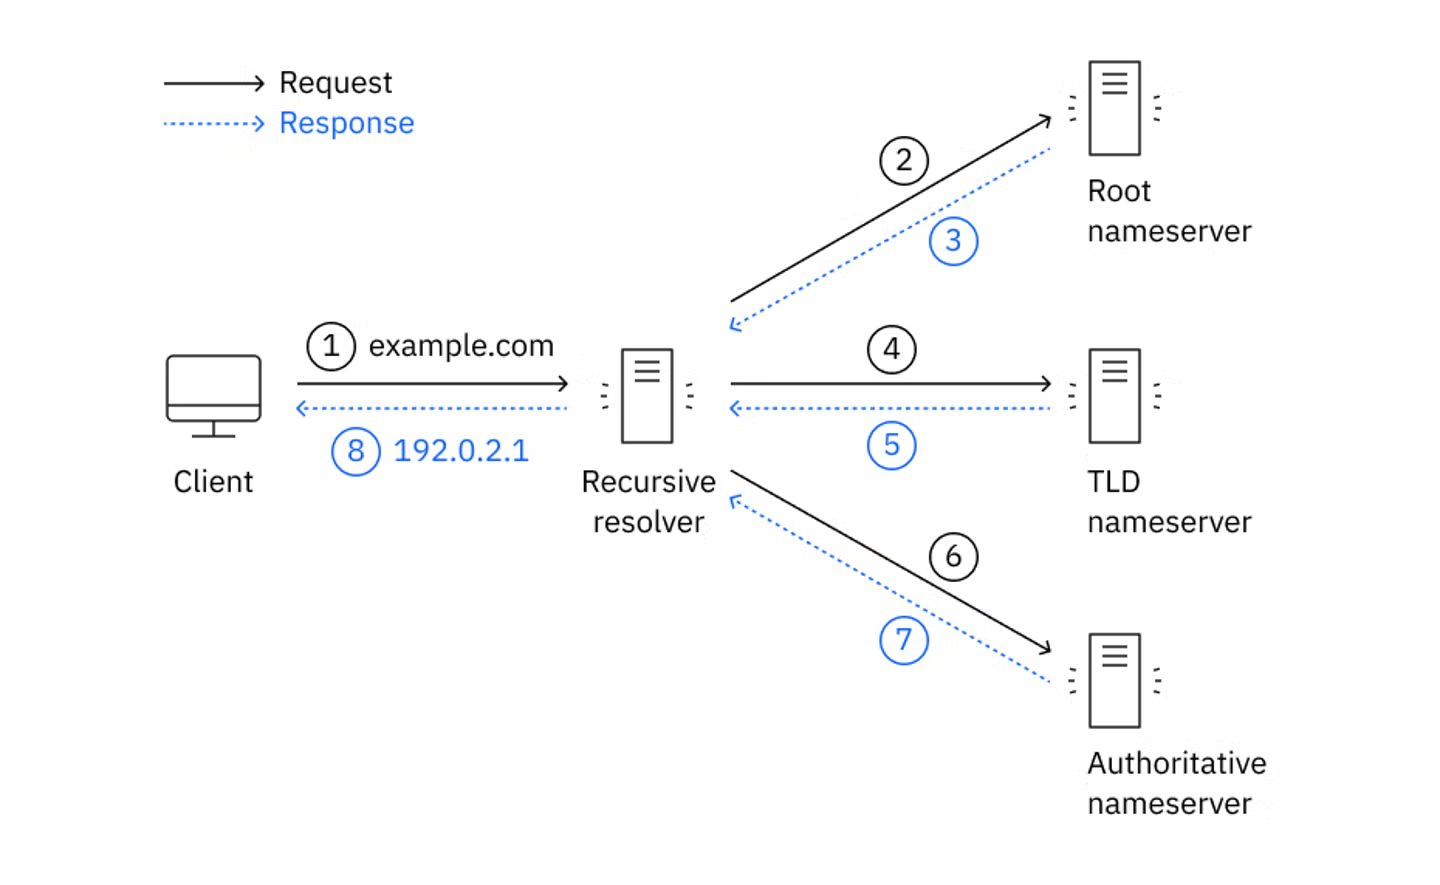
\includegraphics[width=0.8\textwidth]{diagrams_and_images/dns_resolution.png}
	\caption{Exemple simplifié d'une résolution DNS récursive.}
	\label{fig:dns_resolution}
	\end{figure}

	\subsection{Serveurs autoritatifs et résolveurs}

	L'infrastructure DNS est principalement composée de deux types de serveurs.

	Les \textbf{serveurs autoritatifs} stockent les informations officielles relatives à un ou plusieurs domaines. Ils constituent la source de vérité concernant les enregistrements DNS qu'ils hébergent.

	Les \textbf{résolveurs DNS} ont pour rôle de répondre aux requêtes des clients. Lorsqu'une information n'est pas disponible localement, ils interrogent successivement les différents serveurs de la hiérarchie DNS jusqu'à obtenir une réponse qu'ils retransmettent au client.

	Dans le cadre de ce stage, les travaux portent principalement sur les résolveurs DNS, car ils représentent le point d'entrée des requêtes générées par les utilisateurs et intègrent des mécanismes de cache susceptibles d'influencer significativement leur consommation énergétique.

	\subsection{Résolution récursive}

	La résolution récursive correspond au processus par lequel un résolveur recherche une information DNS au nom du client.

	Lorsqu'un utilisateur effectue une requête, celle-ci est transmise à un résolveur. Si la réponse n'est pas déjà disponible dans son cache, le résolveur contacte successivement les serveurs racine, puis les serveurs responsables du domaine de premier niveau (\textit{Top-Level Domain}) concerné, avant d'interroger le serveur autoritatif du domaine recherché.

	Une fois la réponse obtenue, elle est renvoyée au client et peut être conservée temporairement dans le cache du résolveur afin d'accélérer les futures requêtes similaires.

	\subsection{Le mécanisme de cache}

	Le cache constitue un élément fondamental du fonctionnement des résolveurs DNS. Lorsqu'une réponse est obtenue auprès d'un serveur autoritatif, elle est conservée localement pendant une durée définie par son \textit{Time To Live} (TTL).

	Si une requête identique est reçue avant l'expiration de cette durée, le résolveur peut répondre directement à partir du cache sans effectuer de nouvelles communications réseau.

	Ce mécanisme permet de réduire la latence des requêtes, de diminuer la charge des serveurs autoritatifs et de limiter le trafic réseau généré par les résolutions DNS. Dans le cadre de ce stage, l'étude de l'impact énergétique du cache constitue un élément central des expérimentations réalisées.

	\section{Protocoles utilisés}

	Traditionnellement, les échanges DNS utilisent le protocole UDP. Cependant, l'apparition de nouvelles exigences en matière de confidentialité et de sécurité a conduit au développement de protocoles chiffrés tels que DNS over TLS (DoT) et DNS over HTTPS (DoH).

	\subsection{DNS sur UDP}

	Le protocole UDP (\textit{User Datagram Protocol}) est historiquement le mode de transport le plus utilisé pour les requêtes DNS.

	Son principal avantage réside dans sa simplicité : aucune connexion préalable n'est nécessaire entre le client et le serveur, ce qui réduit la surcharge protocolaire et permet d'obtenir de très faibles temps de réponse.

	Cependant, les données sont transmises en clair sur le réseau, ce qui les rend observables par des intermédiaires.

	\subsection{DNS over TLS (DoT)}

	Le protocole DNS over TLS encapsule les échanges DNS dans une connexion TLS.

	Cette approche garantit la confidentialité et l'intégrité des données échangées entre le client et le résolveur. En contrepartie, l'établissement et le maintien de la connexion TLS introduisent un coût supplémentaire en termes de calcul et de consommation de ressources.

	\subsection{DNS over HTTPS (DoH)}

	Le protocole DNS over HTTPS transporte les requêtes DNS au travers du protocole HTTPS.

	En plus du chiffrement apporté par TLS, cette approche permet aux requêtes DNS de se fondre dans le trafic Web classique. Cette caractéristique améliore la confidentialité des utilisateurs mais ajoute également une couche protocolaire supplémentaire susceptible d'avoir un impact sur les performances et la consommation énergétique des serveurs.

	L'une des motivations de ce stage est précisément d'évaluer l'influence de ces différents protocoles sur la consommation des infrastructures DNS.

	\section{Présentation de Bind9}

	Les expérimentations réalisées durant ce stage reposent principalement sur Bind9 (\textit{Berkeley Internet Name Domain}), l'un des logiciels DNS les plus utilisés au monde.

	Développé par l'ISC (\textit{Internet Systems Consortium}), Bind9 est une implémentation open source permettant de déployer aussi bien des serveurs DNS autoritatifs que des résolveurs récursifs. Sa large adoption dans les environnements académiques, industriels et institutionnels en fait une référence pertinente pour l'étude du comportement énergétique des infrastructures DNS.

	Bind9 offre de nombreuses fonctionnalités avancées, notamment la gestion du cache, le support des protocoles DNS modernes tels que DoT et DoH, ainsi que des outils détaillés de supervision et de collecte de statistiques. Ces caractéristiques en font une plateforme particulièrement adaptée à la réalisation de mesures expérimentales et à la construction de modèles de consommation énergétique.

	L'ensemble des mesures et analyses présentées dans les chapitres suivants a ainsi été réalisé à partir de différentes configurations de Bind9 exécutées sur les serveurs du projet DECODES.

	\chapter{Travail réalisé}

	Introduction 

	\section{Description du projet DECODES}
	Décirire le sujet défini à mon arrivée et les objectifs généraux du projet.
	Mon rôle dans le projet.
	(organigramme des gens du projet et de leurs rôles)
	Décrire le sujet réel (analyse de la complexité et modélisation)

	\subsection{Organisation du travail}

	Le stage s'inscrivait dans le cadre du projet DECODES (\textit{Datacenter Energy Consumption Optimisation by DNS EvaluationS}), mené en collaboration avec plusieurs partenaires académiques et industriels, notamment l'AFNIC, IXFrance, l'ENPC et Télécom SudParis.

	L'organisation du travail reposait sur une large autonomie dans la conduite des activités de recherche. Les objectifs généraux étaient définis par les encadrants, mais le choix des méthodologies, des outils et des protocoles expérimentaux relevait en grande partie de mon initiative. Cette liberté m'a permis d'explorer différentes approches et d'adapter progressivement mes travaux en fonction des résultats obtenus.

	Le suivi du stage était assuré au travers de réunions régulières avec mes encadrants, généralement organisées de manière hebdomadaire. Ces échanges permettaient de présenter l'avancement des travaux, de discuter des difficultés rencontrées et d'orienter les prochaines étapes de la recherche.

	J'ai également participé à plusieurs réunions plénières du projet DECODES réunissant l'ensemble des partenaires. Ces rencontres ont constitué une opportunité de présenter les résultats intermédiaires obtenus, de recueillir des retours extérieurs et de mieux comprendre les enjeux globaux du projet.

	Les travaux réalisés au cours du stage se sont articulés autour de quatre grandes phases :

	\begin{enumerate}
		\item \textbf{Étude bibliographique}

		Une première phase a consisté à acquérir une compréhension approfondie du sujet à travers l'étude de la littérature scientifique relative au DNS, aux infrastructures réseau et aux méthodes de mesure de la consommation énergétique.

		\item \textbf{Conception de l'environnement expérimental}

		Cette étape a porté sur la mise en place des outils nécessaires aux expérimentations : développement de scripts de mesure, configuration des serveurs de test et validation des protocoles de collecte de données.

		\item \textbf{Campagnes de mesures et analyse des résultats}

		Les expérimentations ont ensuite été conduites de manière itérative afin d'évaluer différentes configurations et d'améliorer progressivement la qualité des mesures obtenues.

		\item \textbf{Modélisation et valorisation des travaux}

		Enfin, les résultats collectés ont été exploités afin de construire des modèles d'analyse et de documenter les conclusions du stage au travers de rapports, présentations et travaux de rédaction.

	\end{enumerate}

	\section{État de l'art}

	\section{Déroulement du travail}

	\subsection{Conception de l'environnement expérimental}

	La première partie de cette recherche consiste à mesurer de manière efficace et détaillée la consommation d'un résolveur DNS. Pour ce faire, j'ai choisi une approche boîte noire, en mesurant le plus grand nombre de métriques possibles, puis en déduisant celles qui sont les plus pertinentes pour estimer la consommation énergétique.

	\subsubsection{Configuration des différentes machines}

	La configuration se compose d'un client et d'un DNS. Le client agit également comme orchestrateur et lancera les mesures sur les deux machines. La consommation énergétique externe est collectée à l'aide d'un Yoctopuce (wattmètre) et est surveillée par le client.

	Le DNS utilise une implémentation de Bind9.

	le client orchestre les mesures et fait office de client
	Le DNS possede des scripts de mesures de diffétentes metriques (ces scripts consomment, cette consommation ne doit pas etre négilgée )

	\begin{center}
	\begin{tikzpicture}[
		mynode/.style={
			draw,
			rounded corners=5pt,
			minimum width=2cm,
			minimum height=0.8cm,
			align=center,
			inner sep=4pt,
			font=\small,
		},
		myedge/.style={
			line width=1pt,
			rounded corners=8pt,
			>={Stealth[scale=0.8]},
			nodes={fill=white},
		}
	]

		% Couleurs
		\colorlet{color0}{red!30}
		\colorlet{color1}{blue!30}
		\colorlet{color2}{green!30}
		\colorlet{color3}{yellow!30}

		% Noeuds (de gauche à droite)
		\node[mynode, fill=color0] (power) at (0,6) {Source d'alimentation};
		\node[mynode, fill=color1] (yocto) at (0,3) {Yoctopuce};
		\node[mynode, fill=color3] (monitoring) at (10,3) {PC de surveillance};
		\node[mynode, fill=color2] (scripts) at (10,0) {Scripts de mesure};
		\node[mynode, fill=color2] (dns) at (0,0) {DNS};

		% Fond gris pour DNS et scripts de mesure
		\begin{scope}[on background layer]
			\node[fill=gray!50, rounded corners=5pt, fit=(dns) (scripts), inner sep=10pt] {};
		\end{scope}

		% Connexions
		\draw[myedge, ->] (power) -- (yocto) node[midway] {Alimentation};
		\draw[myedge, ->] (yocto) -- (monitoring) node[midway] {USB};
		\draw[myedge, ->] (yocto) -- (dns) node[midway] {Alimentation};
		\draw[myedge, ->] (monitoring) -- (dns) node[midway] {Envoi de requêtes};
		\draw[myedge, ->] (monitoring) -- (scripts) node[midway] {Lance les scripts};

	\end{tikzpicture}
	\end{center}

	\subsubsection{Outils de mesure utilisés}
	Un grand nombre de métriques sont collectées pour aider à estimer et modéliser la consommation énergétique du résolveur DNS. Ces métriques peuvent se classer dans 4 catégories : les mesures de critéres systemes, les mesures de consommation énergétiques externes, les logs réseau et les mesures spécifiques au logiciel (Bind9).
	Pour collecter ces métriques les outils utilisés selon la catégories sont :
	\begin{itemize}
		\item \textbf{Mesures de critères systèmes :} \texttt{turbostat} (CPU), mesures système donées par le kernel (I/O, NIC,), \texttt{perf} (RAM)
		\item \textbf{Mesures de consommation énergétique externes :} \texttt{Yoctopuce}
		\item \textbf{Logs réseau :} \texttt{tcpdump}
		\item \textbf{Mesures spécifiques à Bind9 :} \texttt{rndc} (Informations sur le cache de Bind9), \texttt{uftrace} (Rapports des fonctions exécutées par Bind9)
	\end{itemize}

	Les outils de mesures de critères systèmes ont été sélectionnés à l'aide d'un rapport de stage écrit par une étudiante ayant fait une étude comparative de différents outils de mesure de consommation énergétique de serveurs \cite{EnergyMeasurementTools}. Le détail des métriques collectées par ces outils est présenté dans les annexes.
	
	Concernant les outils de mesure spécifiques à Bind9, \texttt{rndc} est un outil de contrôle de Bind9 qui permet d'obtenir des informations sur le cache, les statistiques de requêtes, etc. \texttt{uftrace} est un outil de traçage de fonctions qui permet d'obtenir des rapports détaillés sur les fonctions exécutées par des logiciels comme Bind9, ce qui est particulièrement utile pour l'analyse de la complexité algorithmique.
	
	\subsubsection{Scripts de mesure développés}
	Un script par outil utlisé globalement + différents 

	\emph{Petite conclusion :} Très utile pour les modèles, cela servira de base pour ceux-ci / fournir les données aux constantes, etc.

	
	\subsubsection{Sélection de l'ensemble des noms de domaines utilisés}
	
	Pour faire les mesures de consommation du DNS, il faut envoyer des requêtes de résolution de noms de domaines. Un ensemble de 17 millions de noms de domaine est accéssible sur github avec leur popularité. 
	
	\begin{figure}[H]
		\centering
		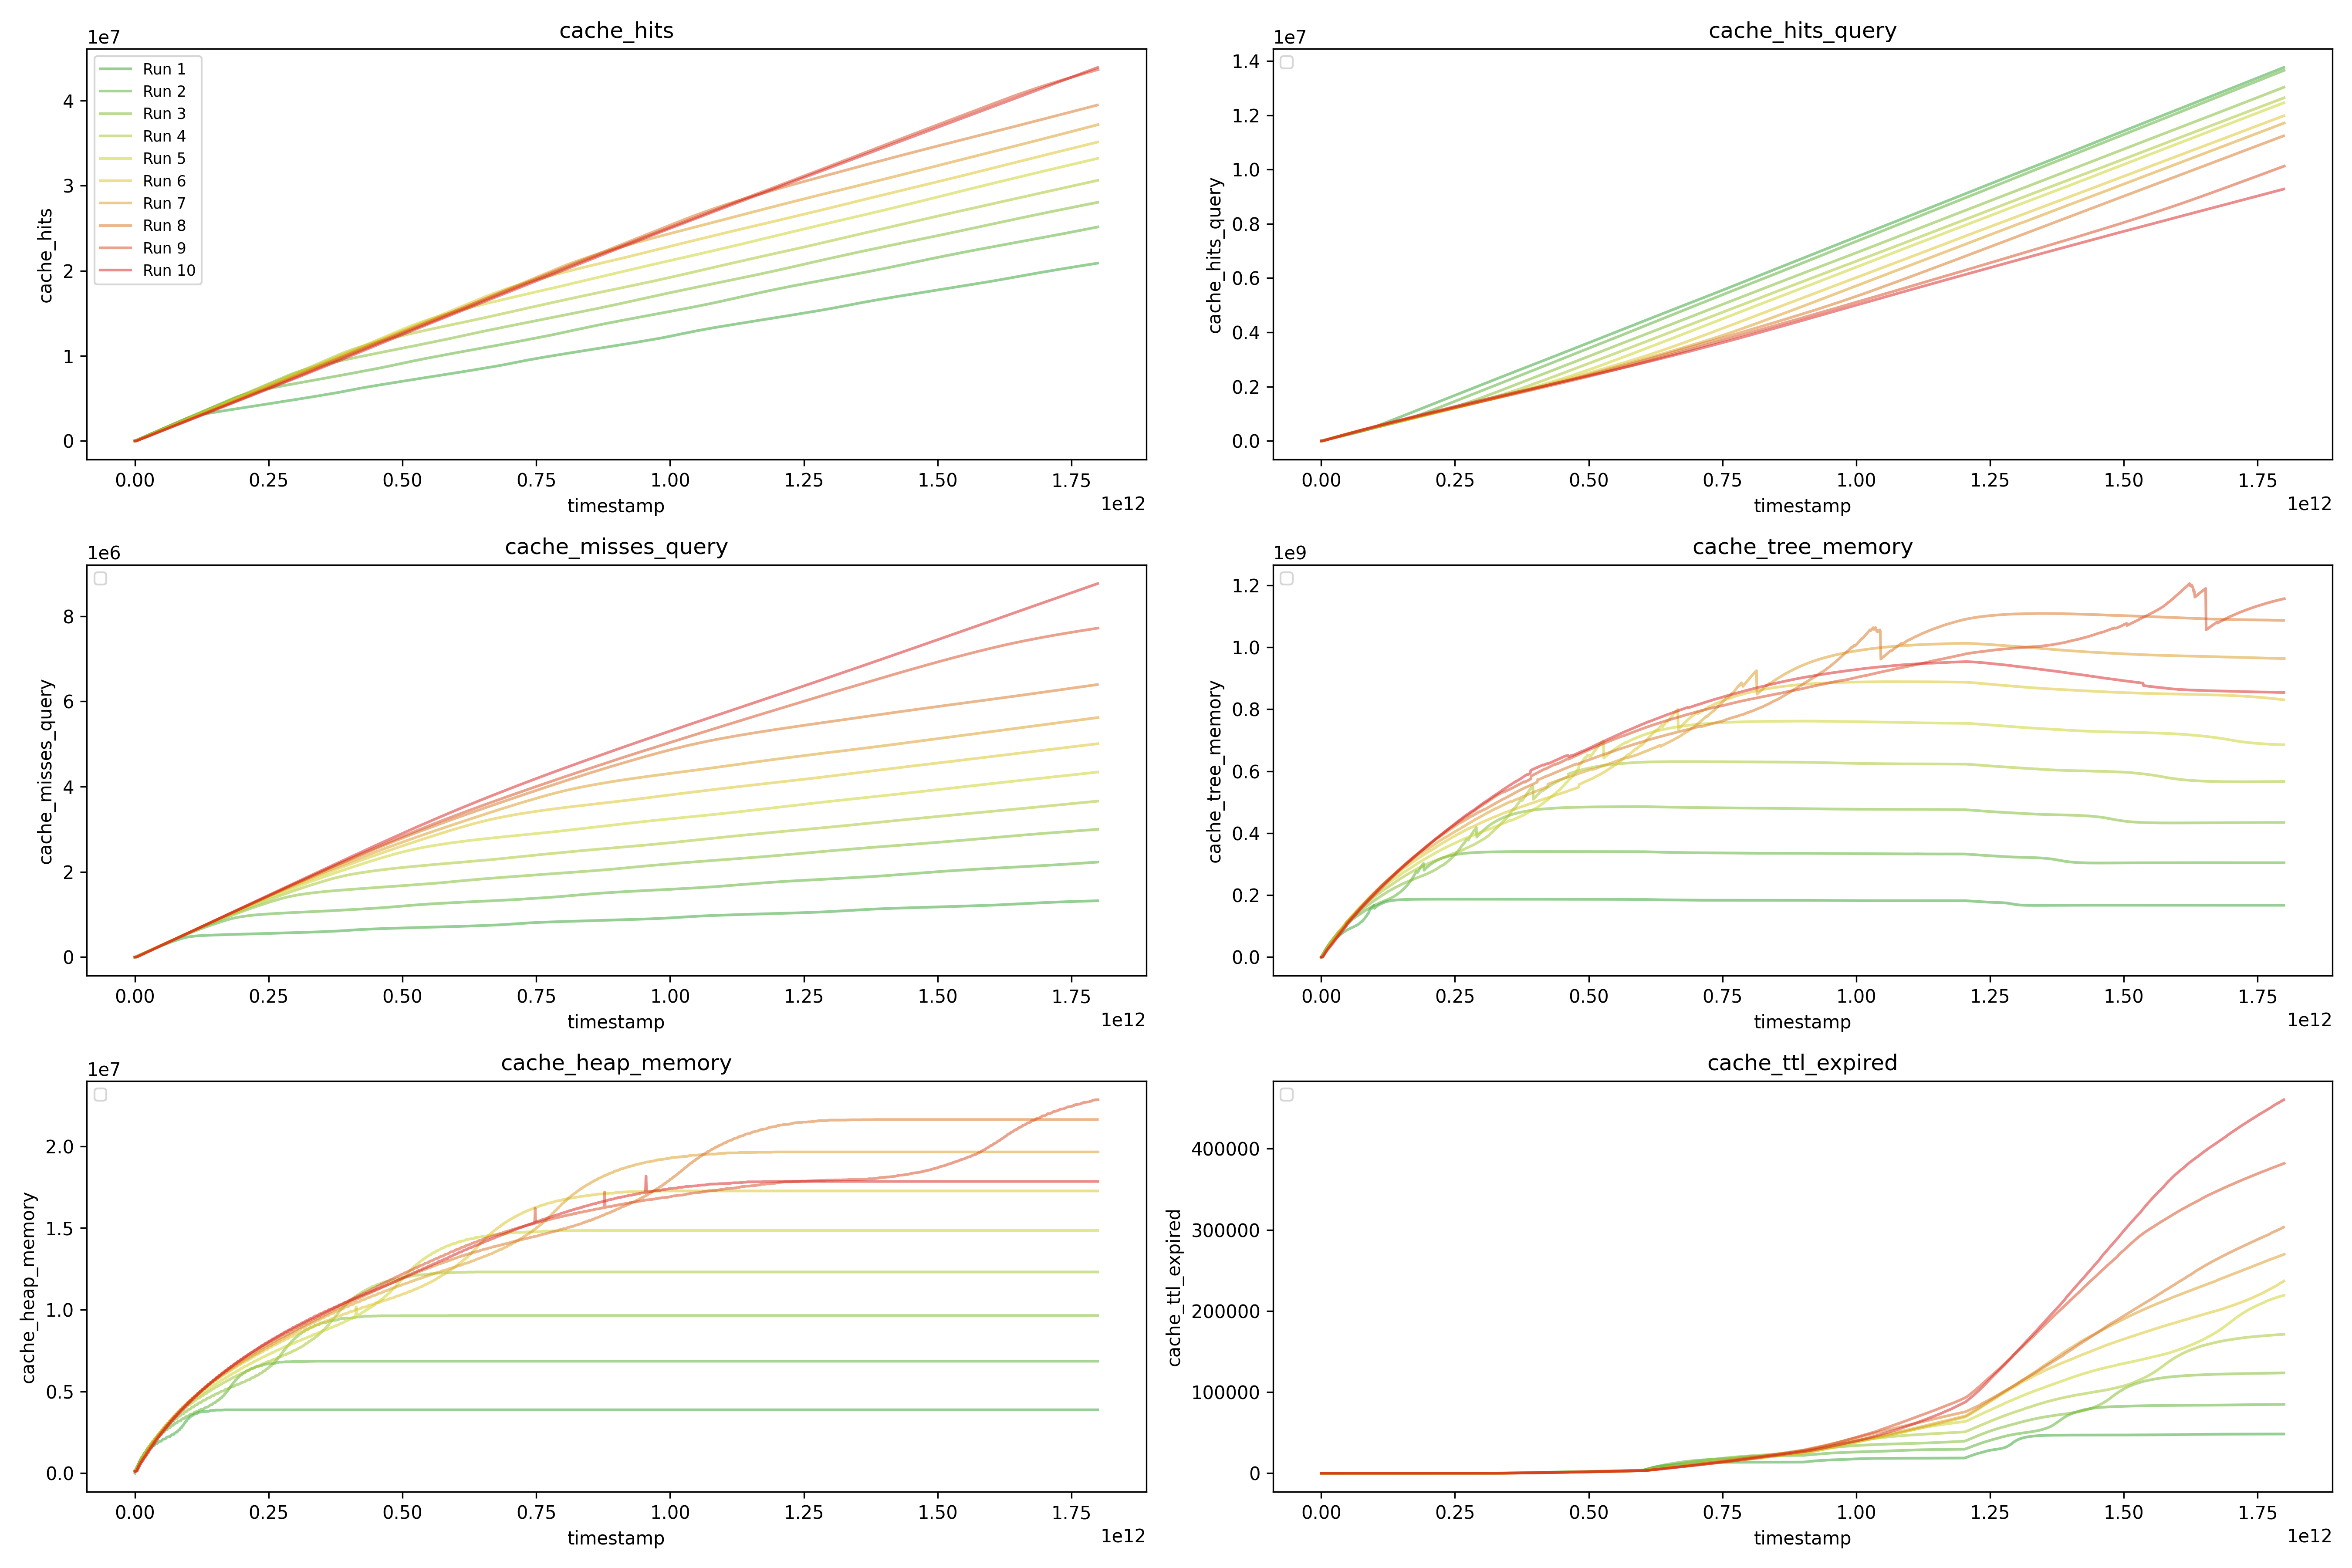
\includegraphics[width=0.9\textwidth]{Graphs/cache_metrics_10.png}
		\caption{Évolution des valeurs associées au cache de bind pour différents ensemble de noms de domaines entre 100 000 et 1 millions de noms de domaines}
		\label{fig:Evolution du cache 1M}
	\end{figure}
	\begin{figure}[H]
		\centering
		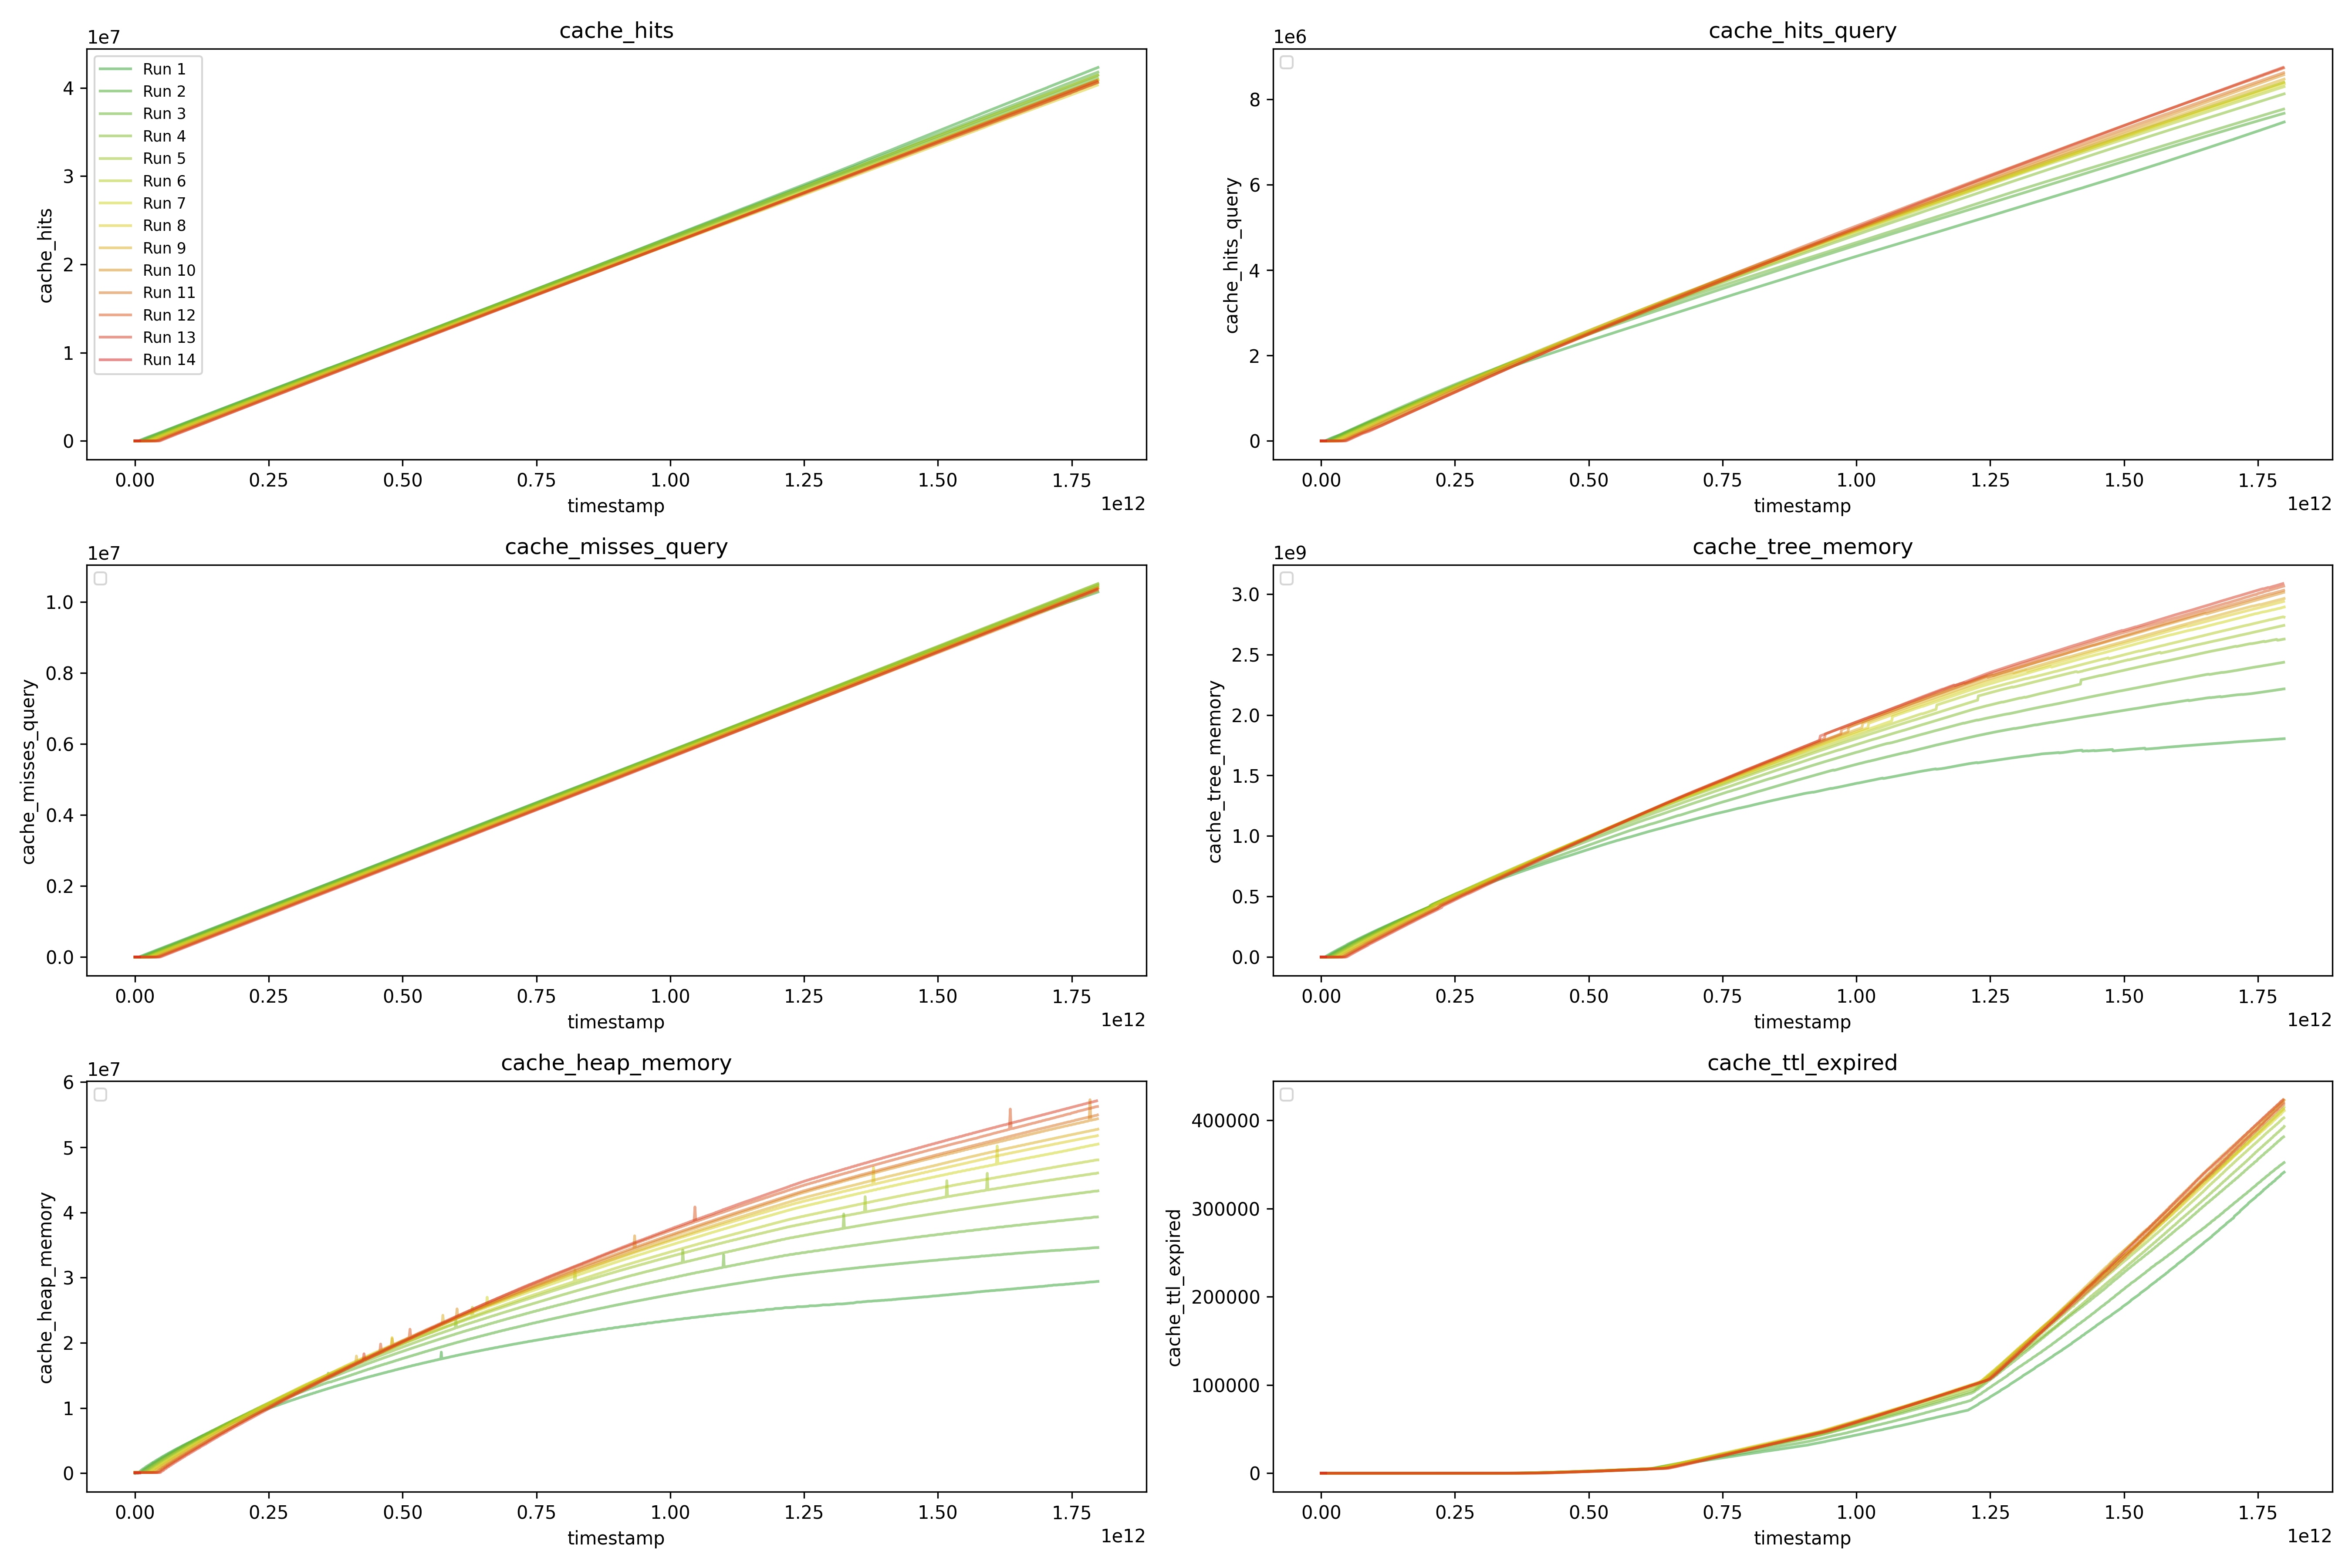
\includegraphics[width=0.9\textwidth]{Graphs/cache_metrics_14M.png}
		\caption{Évolution des valeurs associées au cache de bind pour différents ensemble de noms de domaines entre 1 et 14 millions de noms de domaines}
		\label{fig:Evolution du cache 14M}
	\end{figure}
	
	
	\subsubsection{Gestion des mesures avec et sans cache}

	\subsection{Campagnes de mesures}
	Décrire les outils utilisés, les scripts de mesures créés, les différentes configurations testées, les problèmes rencontrés et comment ils ont été résolus. 
	Diagrammes détaillés d'un cycle de mesure 
	Estimation de temps pour chaque cycle de mesure
	Sanity check 

	\subsubsection{Mesures de consommation énergétique}
	problemes rencontrés :
	- espace disque insufisant
	- Durée des mesures important (pas vraiment un problème)
	\subsubsection{Mesures de la complexité algorithmique}


	\subsection{Analyse des résultats}

	Les mesures obtenues ont étés analysées principalement avec des jupyter notebooks en utilisant pandas, numpy et matplotlib pour visualiser les résultats. 

	Ces analyses ont pour but de vérifier des hypothèses émises. La visualisation est essentielle pour valider ces hypothèses et comprendre les résultats obtenus, et repérer les erreurs et anomalies dans les mesures. 

	Certains problemes ont été rencontrés lors de l'analyse des résultats, notamment en raison du temps de traitement nécessaire, et la mémoire vive nécessaire pour analyser les grandes quantités de données collectées. Pour résoudre ce problème, des techniques d'échantillonnage ont été utilisées afin de réduire la taille des ensembles de données tout en conservant une représentativité suffisante pour les analyses. Cela réduit la précision des résultats, mais permet d'obtenir des analyses plus rapidement et de manière plus efficace. Un script a été développé pour automatiser ce processus d'échantillonnage et d'exportation des données dans un format plus facilement manipulable pour les analyses. Il rassemble toutes les métriques collectées lors des mesures, rééchantillone les données a une granularité de 1 seconde, remplit les données manquantes avec une méthode appropriée à la nature des données et les exporte dans un format CSV pour une utilisation ultérieure dans les notebooks d'analyse.

	Grace à ce prétraitement des données automatisé, les résultats suivant ont pu être obtenus et analysés efficacement. 
	
	Le grand nombre de métriques collectées permet de faire des analyses approfondies des différents levier de consommation. Cependant, durant ce stage, ce grand panel de métriques n'a pas été exploité à son plein potentiel et par moment, il a été difficile de trouver quelles étaient les métriques les plus pertinentes à étudier pour ce sujet de recherche.

	Cette section résume les résultats les plus intéressants obtenus et les analyses, en mentionant les limitations de ces résultats s'il y en a, et les prochaines étapes pour les améliorer ou les approfondir.

	\subsubsection{Mesures de consommation énergétique du résolveur DNS}
	
	Les résultats les plus concrets de cette étude de consommation énergétique du résolveur DNS sont ceux montrant la consommation énergétique du résolveur pour les différents protocoles utilisés (UDP, DoT et DoH) avec et sans utilisation du cache pour différentes charges.
	
	Pour les protocols DoT et DoH, les mesures ont été réalisées avec des connexions persistantes et non persistantes. Pour les connexions persistantes, une connexion TLS est établie au début de la mesure et est maintenue tout au long de la mesure. Pour les connexions non persistantes, une nouvelle connexion TLS est établie pour chaque requête DNS envoyée par le client.
	
	Il faut noter que pour DoH, les connxions sont systématiquement persistantes, car DoH utilise le protocole HTTP qui est conçu pour maintenir des connexions persistantes. Cependant, pour les besoins de cette étude, une configuration a été mise en place pour simuler des connexions non persistantes en fermant la connexion HTTP après chaque requête DNS. Cela permet de simuler le fait que chaque requête DoH correspond à un client différent.
	
	
	\begin{figure}[H]
		\centering
		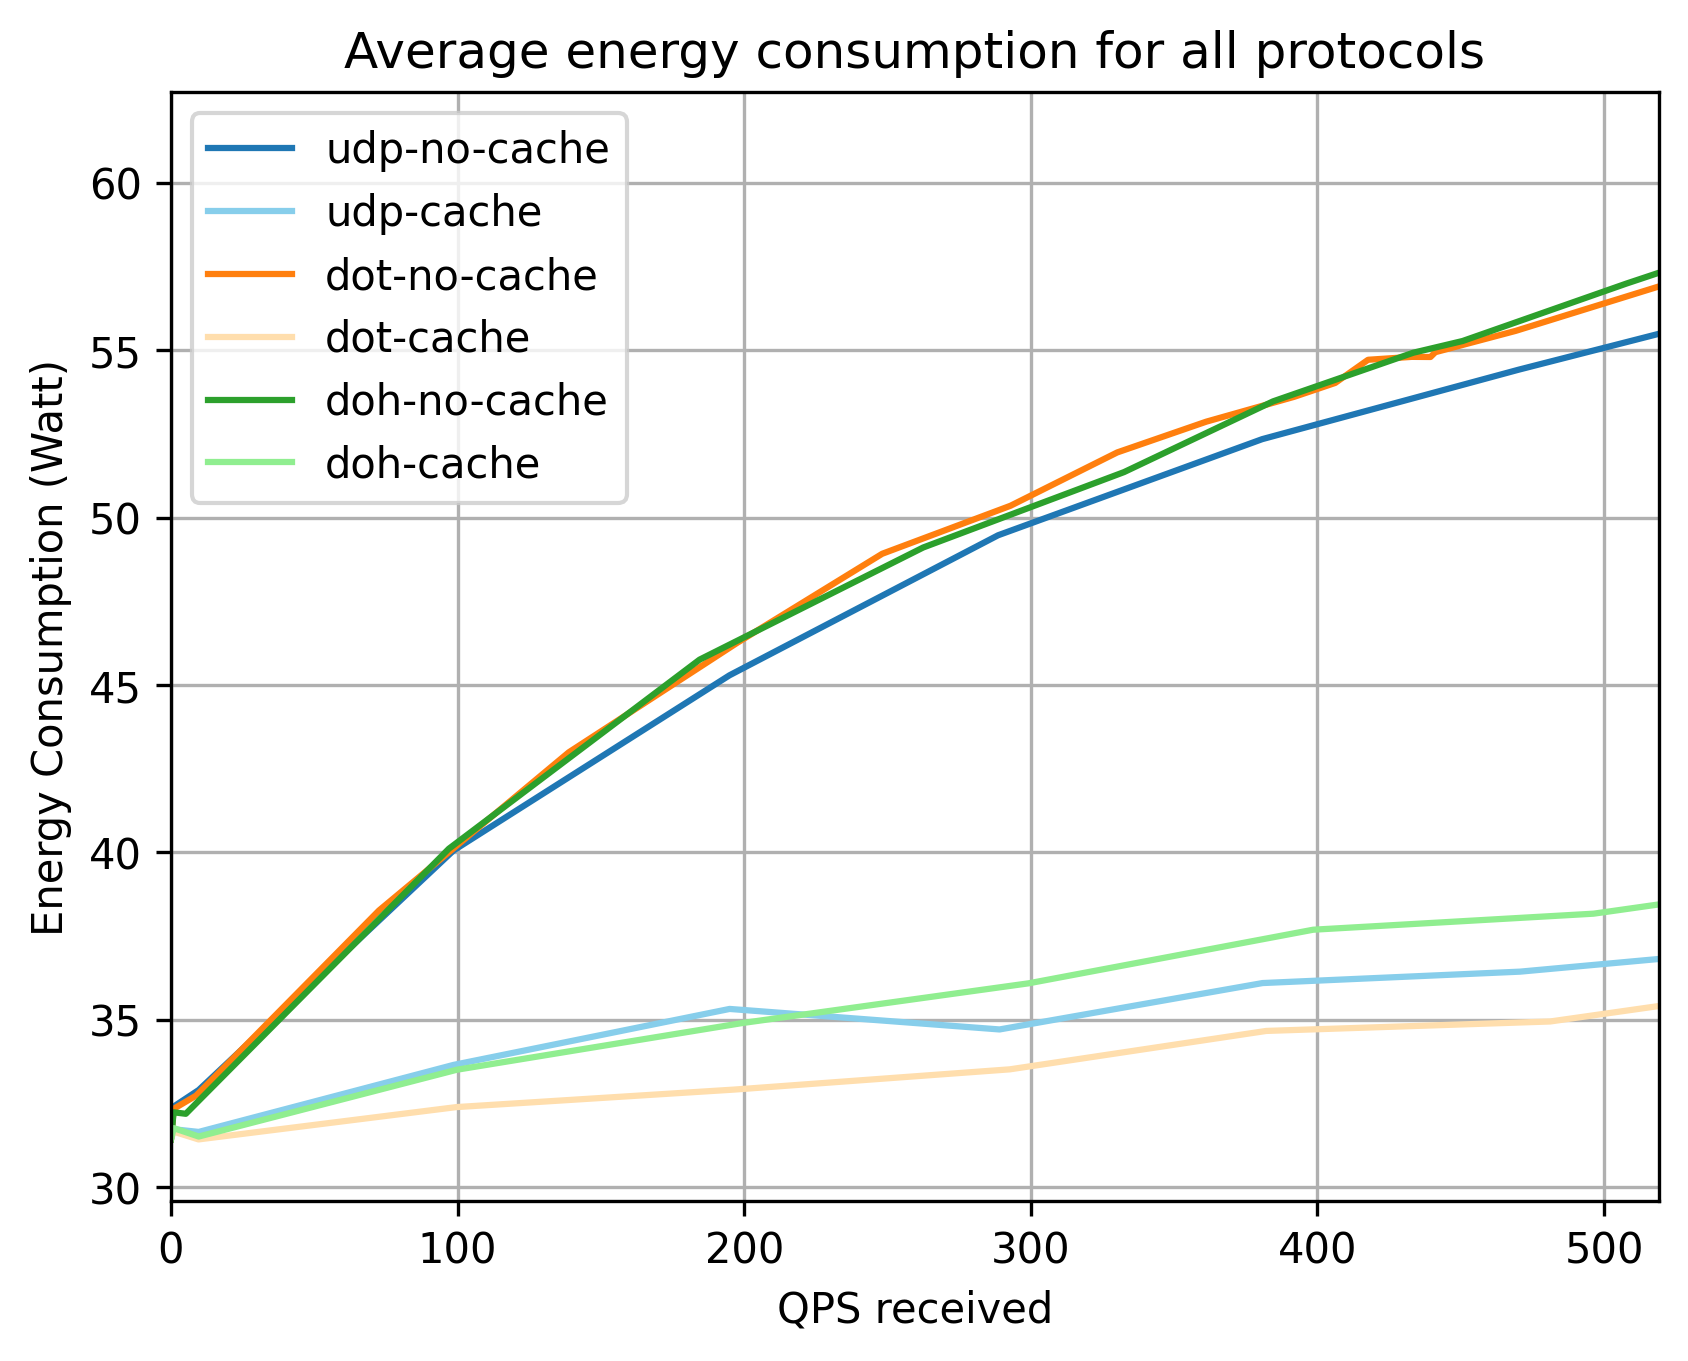
\includegraphics[width=0.9\textwidth]{Graphs/combined_energy_consumption.png}
		\caption{Consommation énergétique moyenne pour UDP, DoT et DoH avec et sans utilisation du cache avec des connexions persistantes}
		\label{fig:consomation_persistante}
	\end{figure}
	
	Il existe une différence claire de consommation énergétique entre l'utilisation avec et sans cache. Les courbes pour l'utilisation sans cache ont une forme de décroissance exponentielle. En observant les courbes d'utilisation du cache, l'ordre est étrange : UDP n'utilise aucune connexion, il devrait donc être en dessous de toutes les autres courbes. 
	
	La différence entre les protocoles utilisant TLS (DoT et DoH) et le protocole utilisant UDP est du au coût du chiffrement principalement. Étant donné que pour ces mesures, les connexions sont persistantes, le coût de l'établissement de la connexion s'efface sur une longue période. Ces résultats sont donc cohérents avec ce qui est attendu. 
	
	Pour voir le coût de l'établissement des connexions, il faut faire des mesures avec des connexions non persistantes.
	
	\begin{figure}[H]
		\centering
		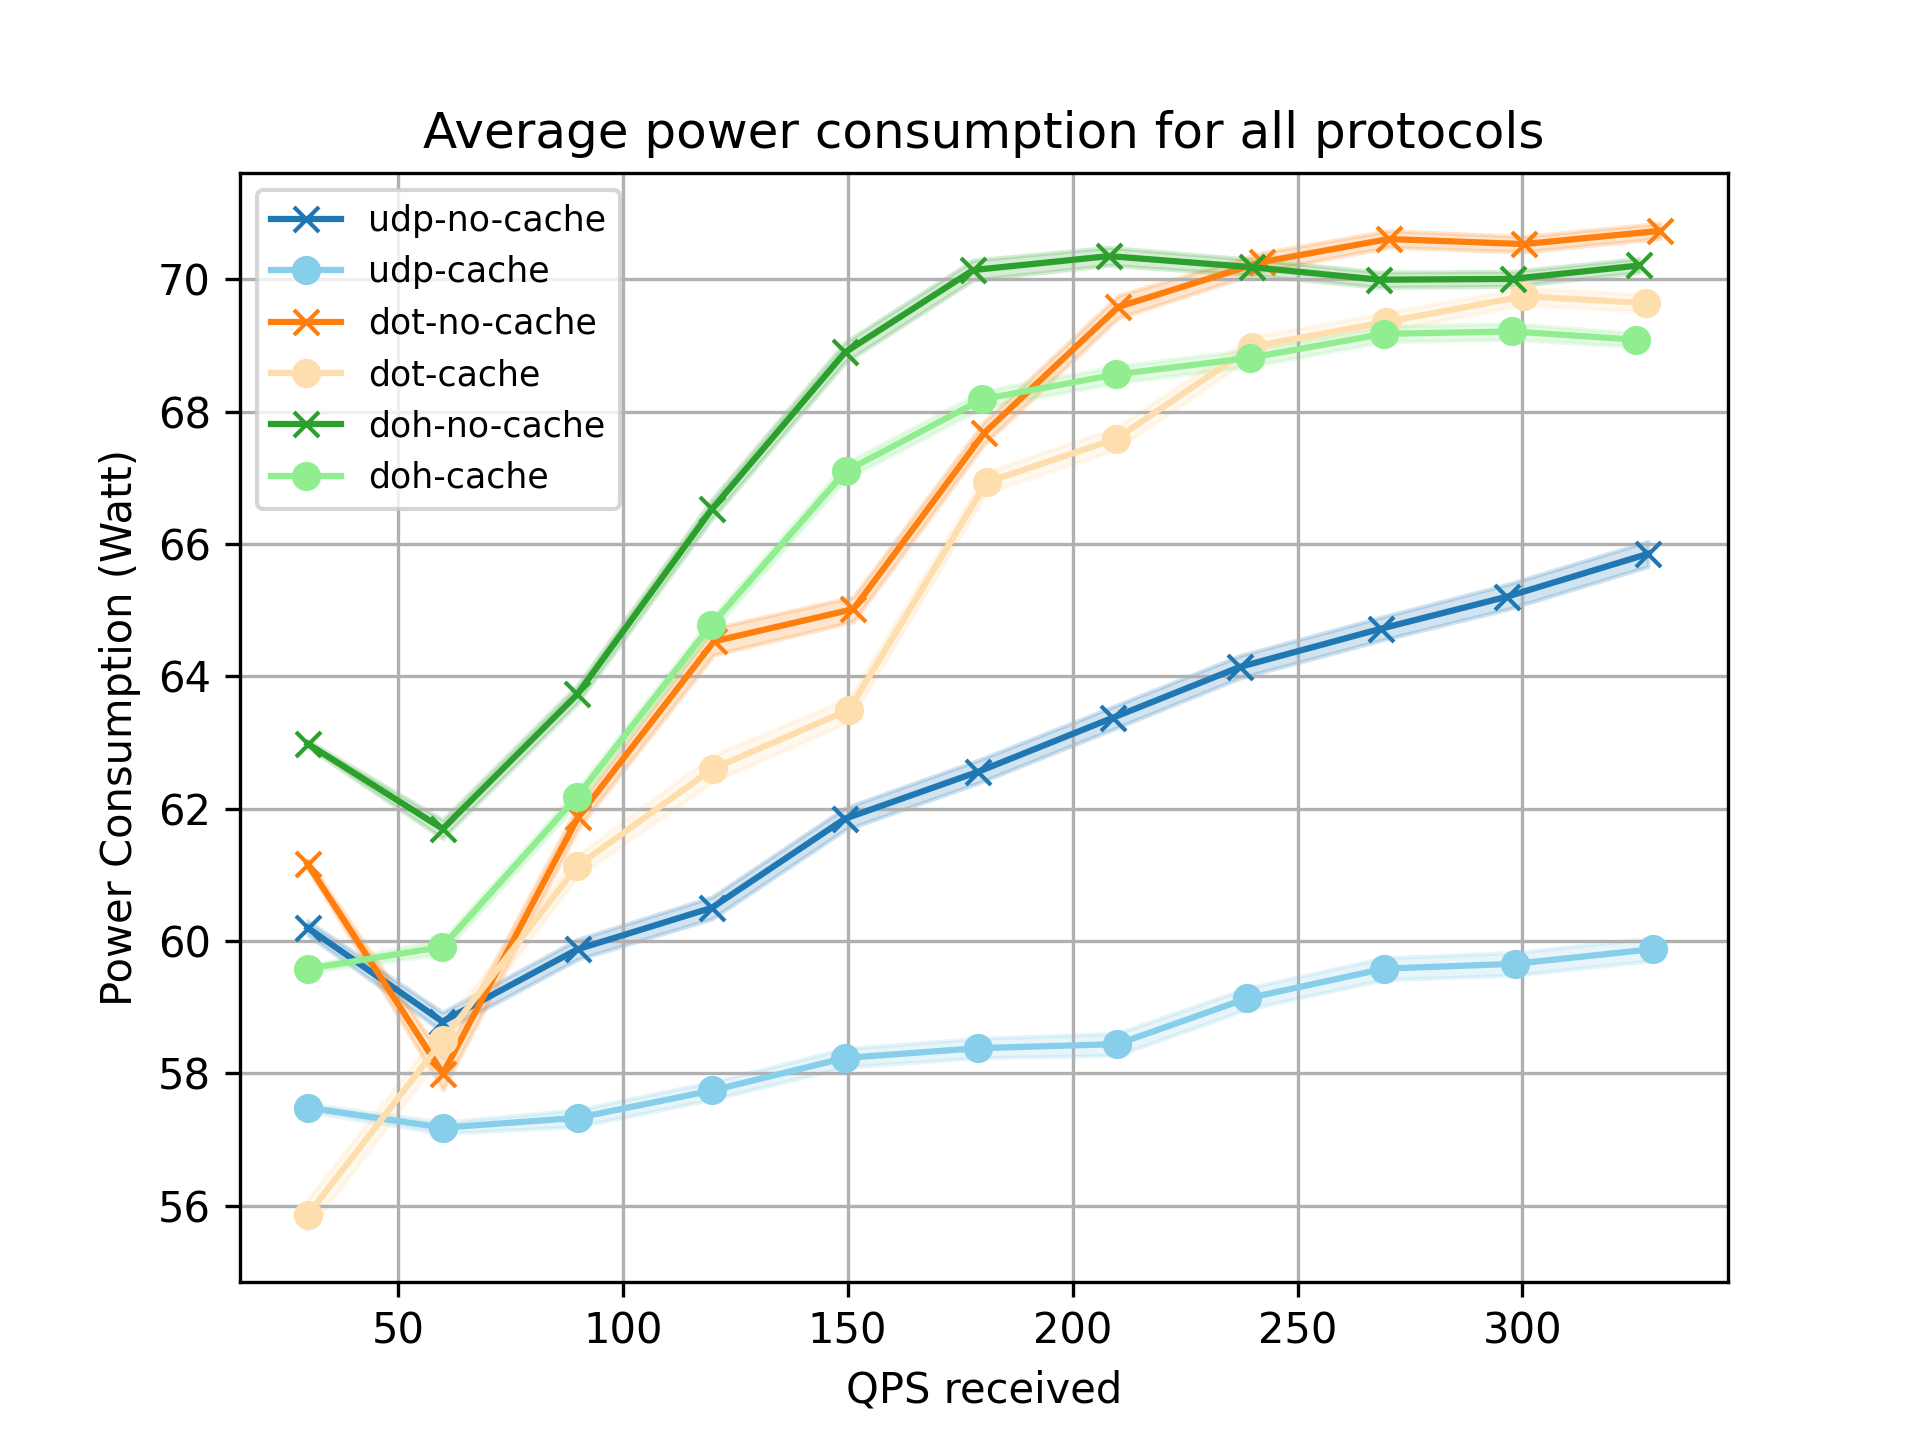
\includegraphics[width=0.9\textwidth]{Graphs/combined_power_consumption_CI_fillbetween.png}
		\caption{Consommation énergétique moyenne pour UDP, DoT et DoH avec et sans utilisation du cache avec des connexions non persistantes}
		\label{fig:consomation_non_persistante}
	\end{figure}

	Avec des connexions non persistantes, la consommation énergétique est plus élevée pour les protocoles utilisant TLS (DoT et DoH) en raison du coût de l'établissement de la connexion pour chaque requête. Le protocol DoH consomme le plus ce qui est cohérent avec le coût supplémentaire du protocole HTTP en plus du chiffrement TLS. 
	
	Pour pourvoir interpréter ces résultats sans biais lié à la surcharge introduite par les scripts de mesure, il est nécessaire de faire des mesures de consommation énergétique sans la surcharge liée à l'enregistrement des métriques au niveau du DNS. 
	
	\begin{figure}[H]
		\centering
		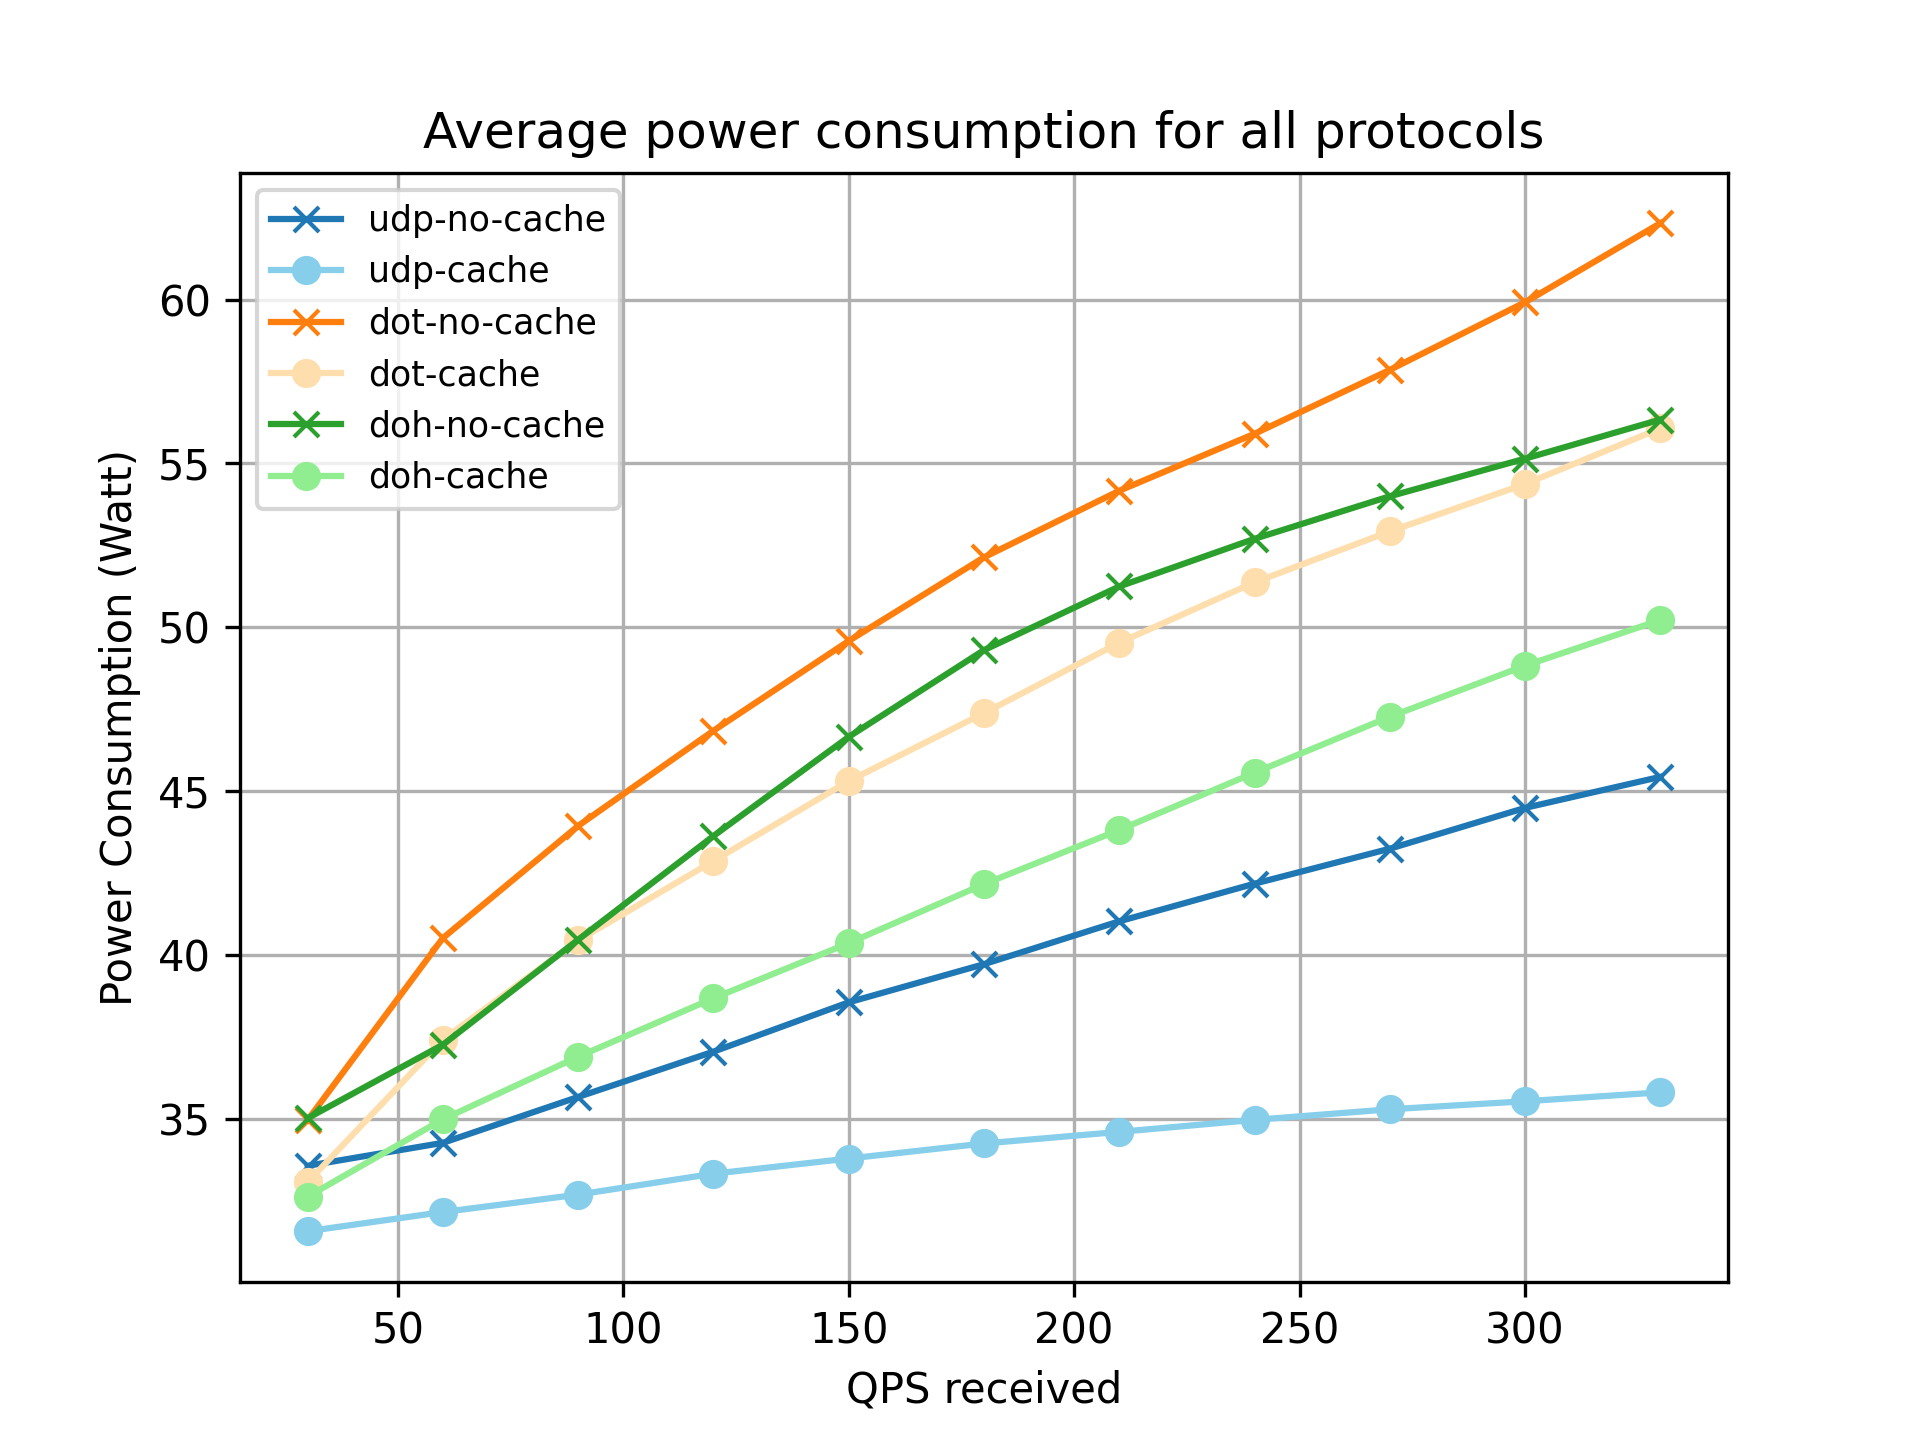
\includegraphics[width=0.9\textwidth]{Graphs/external_measures_consumption.png}
		\caption{Consommation énergétique moyenne pour UDP, DoT et DoH avec et sans utilisation du cache avec des connexions non persistantes, sans la surcharge lié à l'enregistrement des métriques au niveau du DNS}
		\label{fig:consomation_non_persistante_externe}
	\end{figure}

	Étonnamment, les résultats sont différents, le protocole DoT consomme davantage que le protocole DoH, ce qui ne corrobore pas l'hypothèse selon laquelle DoH consomme plus que DoT en raison du coût supplémentaire du protocole HTTP. Comme le protocole mesuré était le même dans ces essais, cette différence provient probablement de la consommation des scripts de mesure au niveau du DNS, qui dépend donc du protocole utilisé. 
	
	Le QPS est limité pour DoT et DoH en raison de la surcharge introduite par l'établissement de connexions TLS pour chaque requête, ce qui rend les mesures à des QPS plus élevés difficiles à réaliser. De plus, il y a un nombre limité de socket disponibles pour les connexions TLS, ce qui peut également limiter la capacité à atteindre des QPS plus élevés. C'est encore plus flagrant avec les connexions non persistantes, où une nouvelle connexion TLS doit être établie pour chaque requête. DoH est le protocol avec le plus de surcharge, par conséquent, c'est le protocol avec lequel le QPS maximum est le plus bas.
	
	Il serait intéressant d'avoir des mesures pour des QPS plus élevés et avec différentes configurations DNS (nombre maximal de clients du résolveur, nombre de threads de travail, etc.) et différentes implémentations DNS (PowerDNS, Unbound, Knot DNS, etc.).
	
	
	---
	\subsubsection{Densité de la consommation énergétique}

	Afin de visualiser la consommation énergétique du résolveur et sa distribution, voici 3 graphiques montrant la distribution de la consommation énergétique lors de l'utilisation du cache et sans utilisation du cache.
	
	\begin{figure}[H]
		\centering
		\begin{minipage}{0.3\textwidth}
			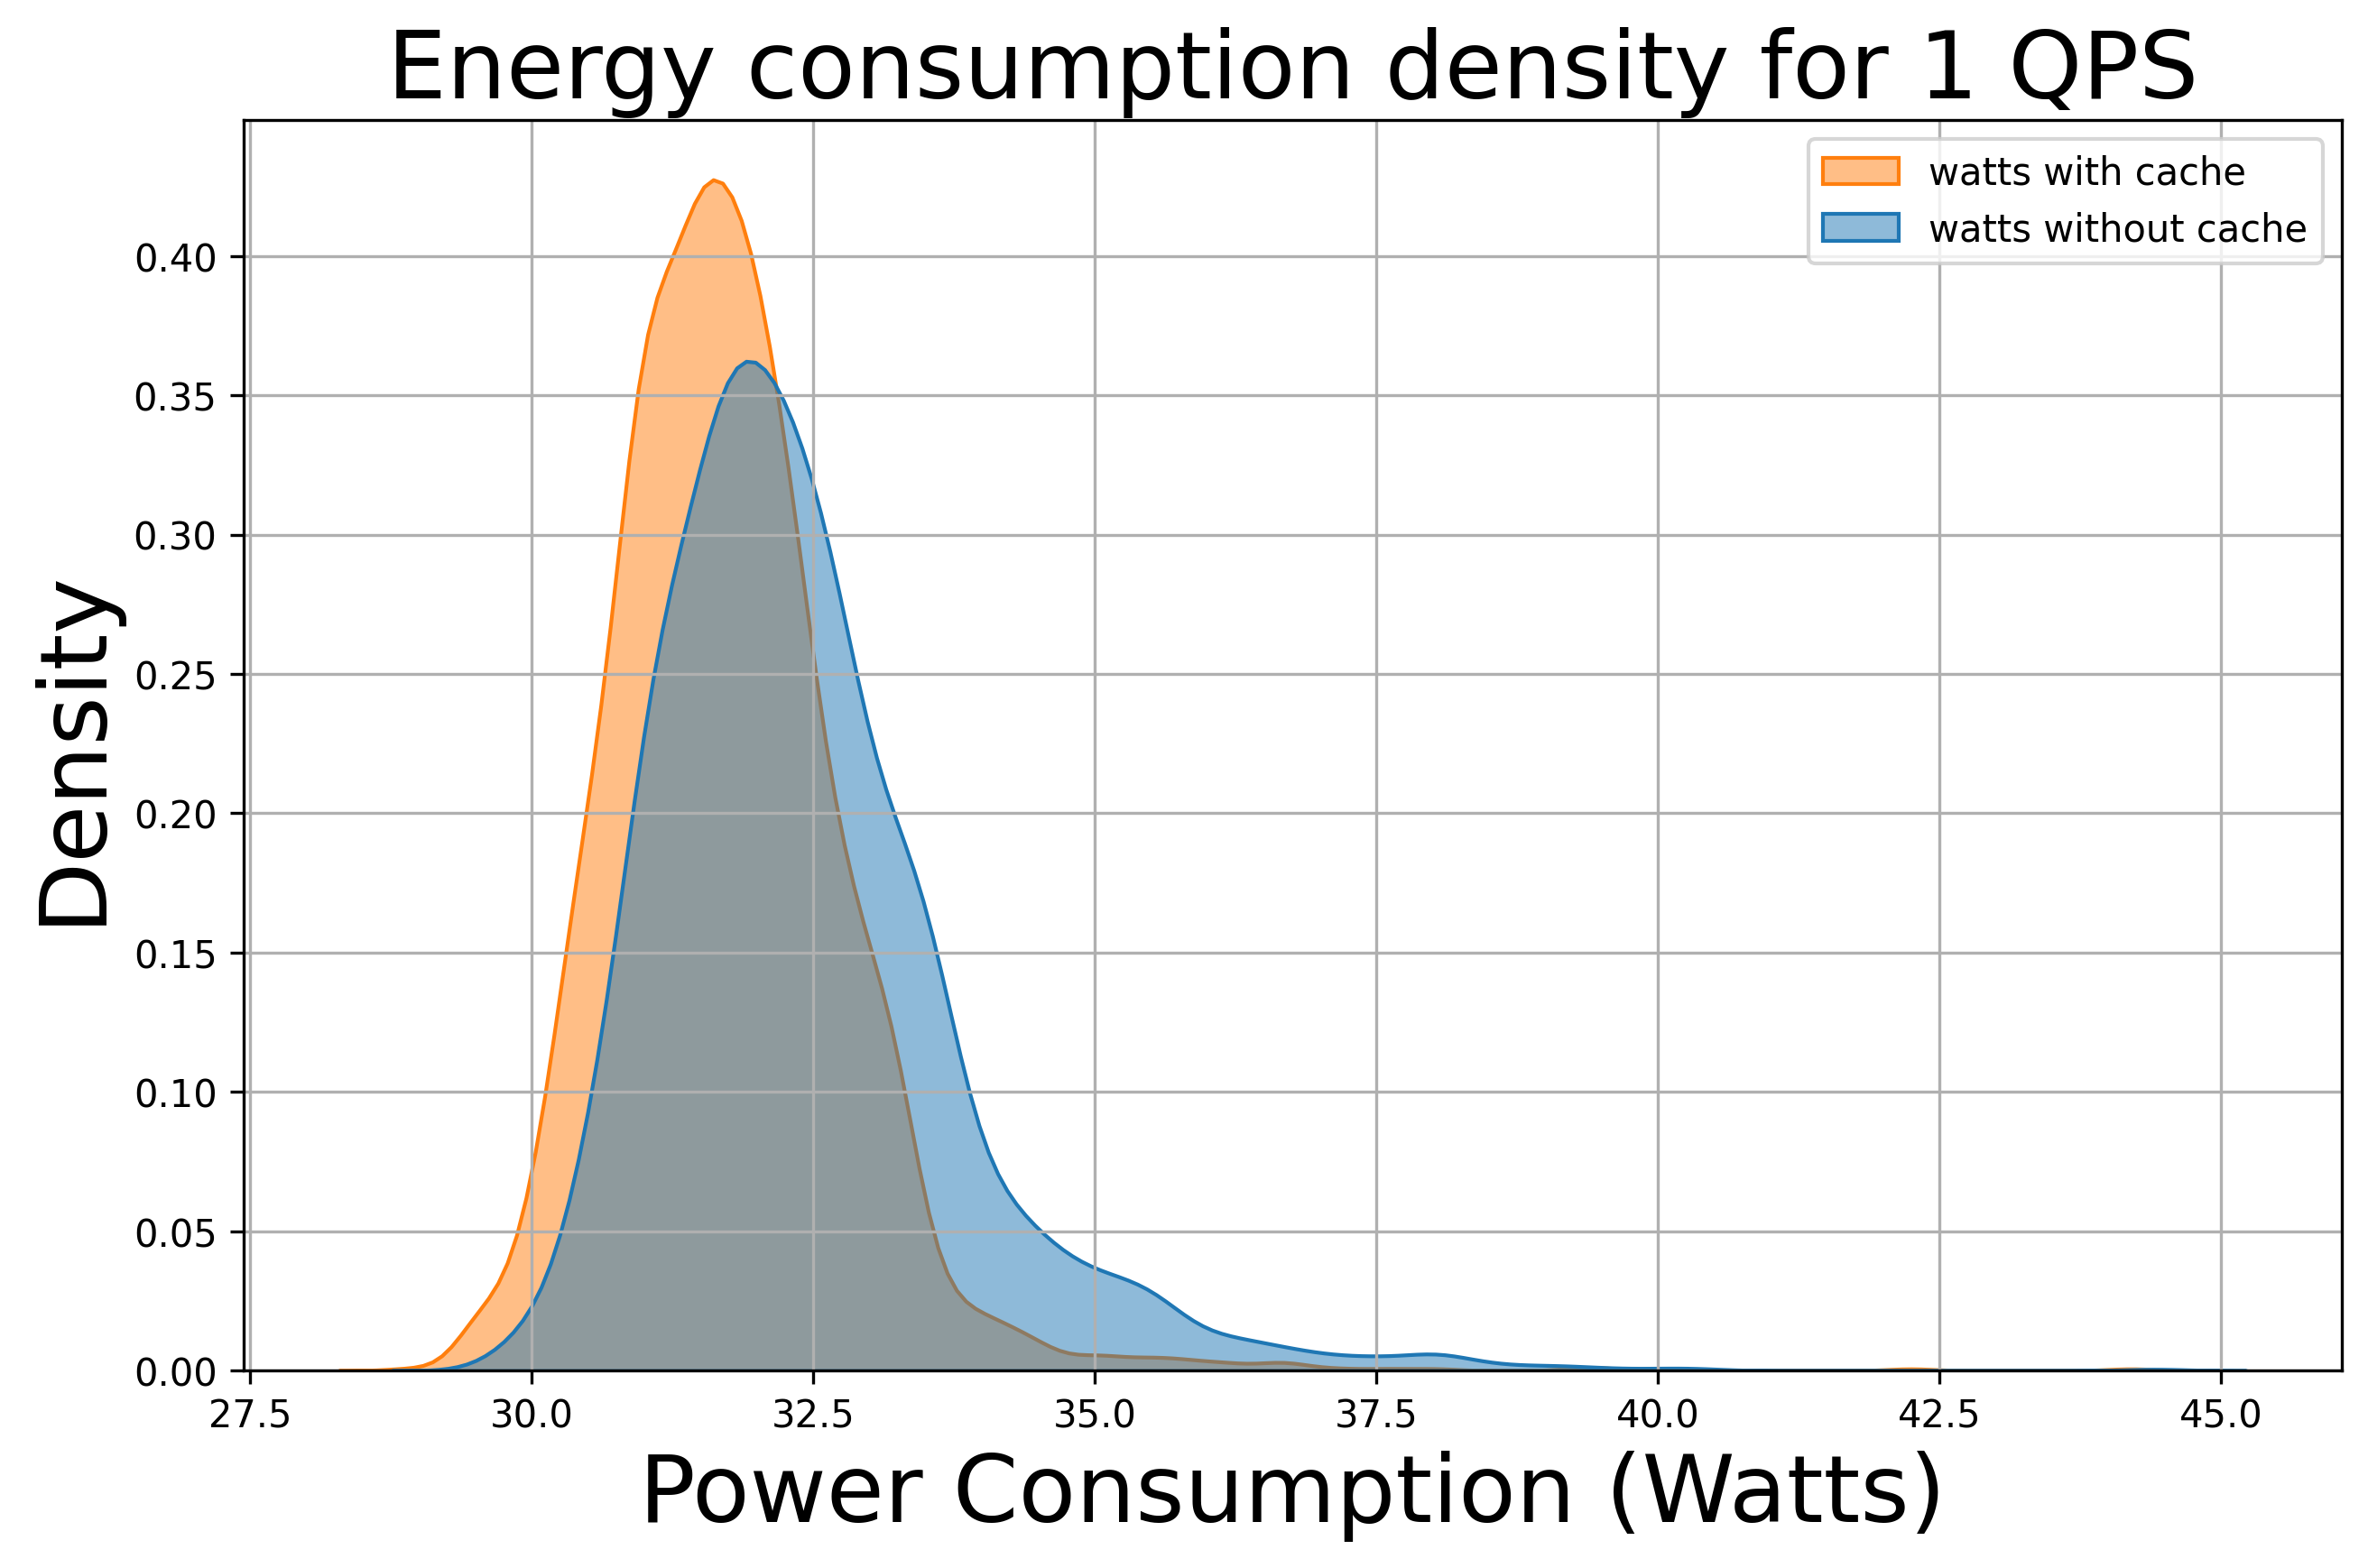
\includegraphics[width=\textwidth]{Graphs/consumption_density_qps_1_udp.png}
		\end{minipage}
		\hfill
		\begin{minipage}{0.3\textwidth}
			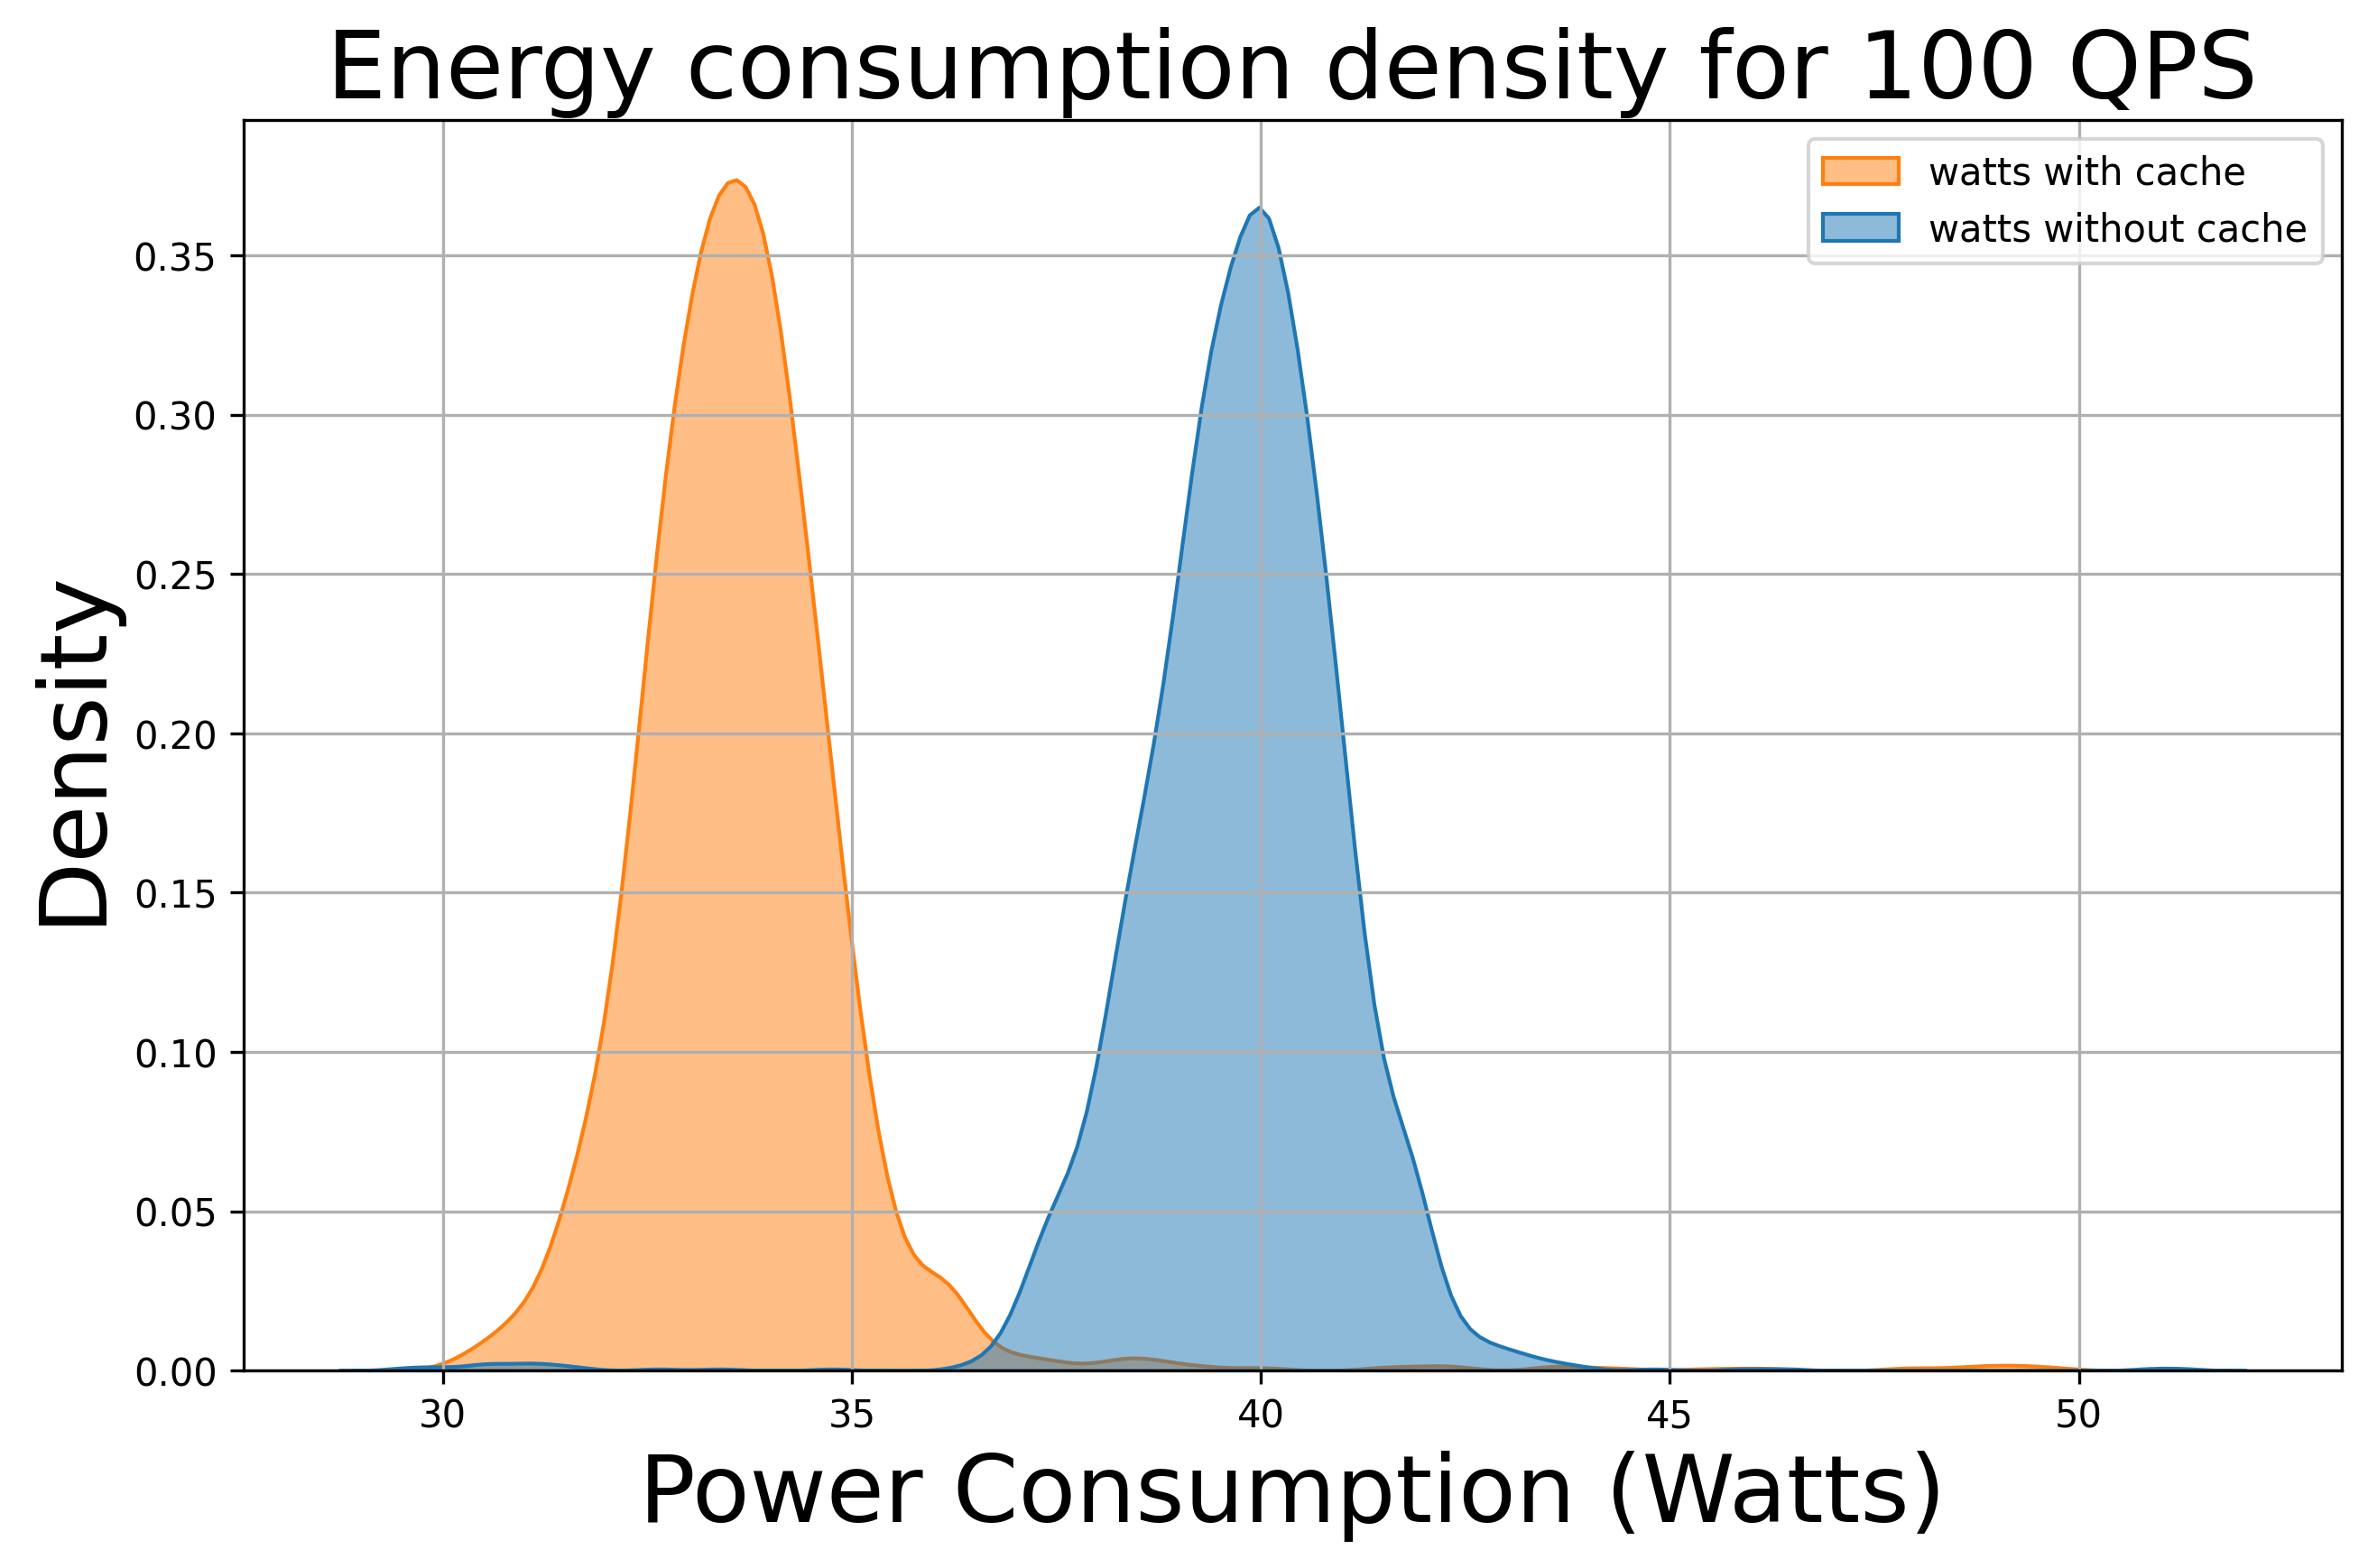
\includegraphics[width=\textwidth]{Graphs/consumption_density_qps_100_udp.png}
		\end{minipage}
		\hfill
		\begin{minipage}{0.3\textwidth}
			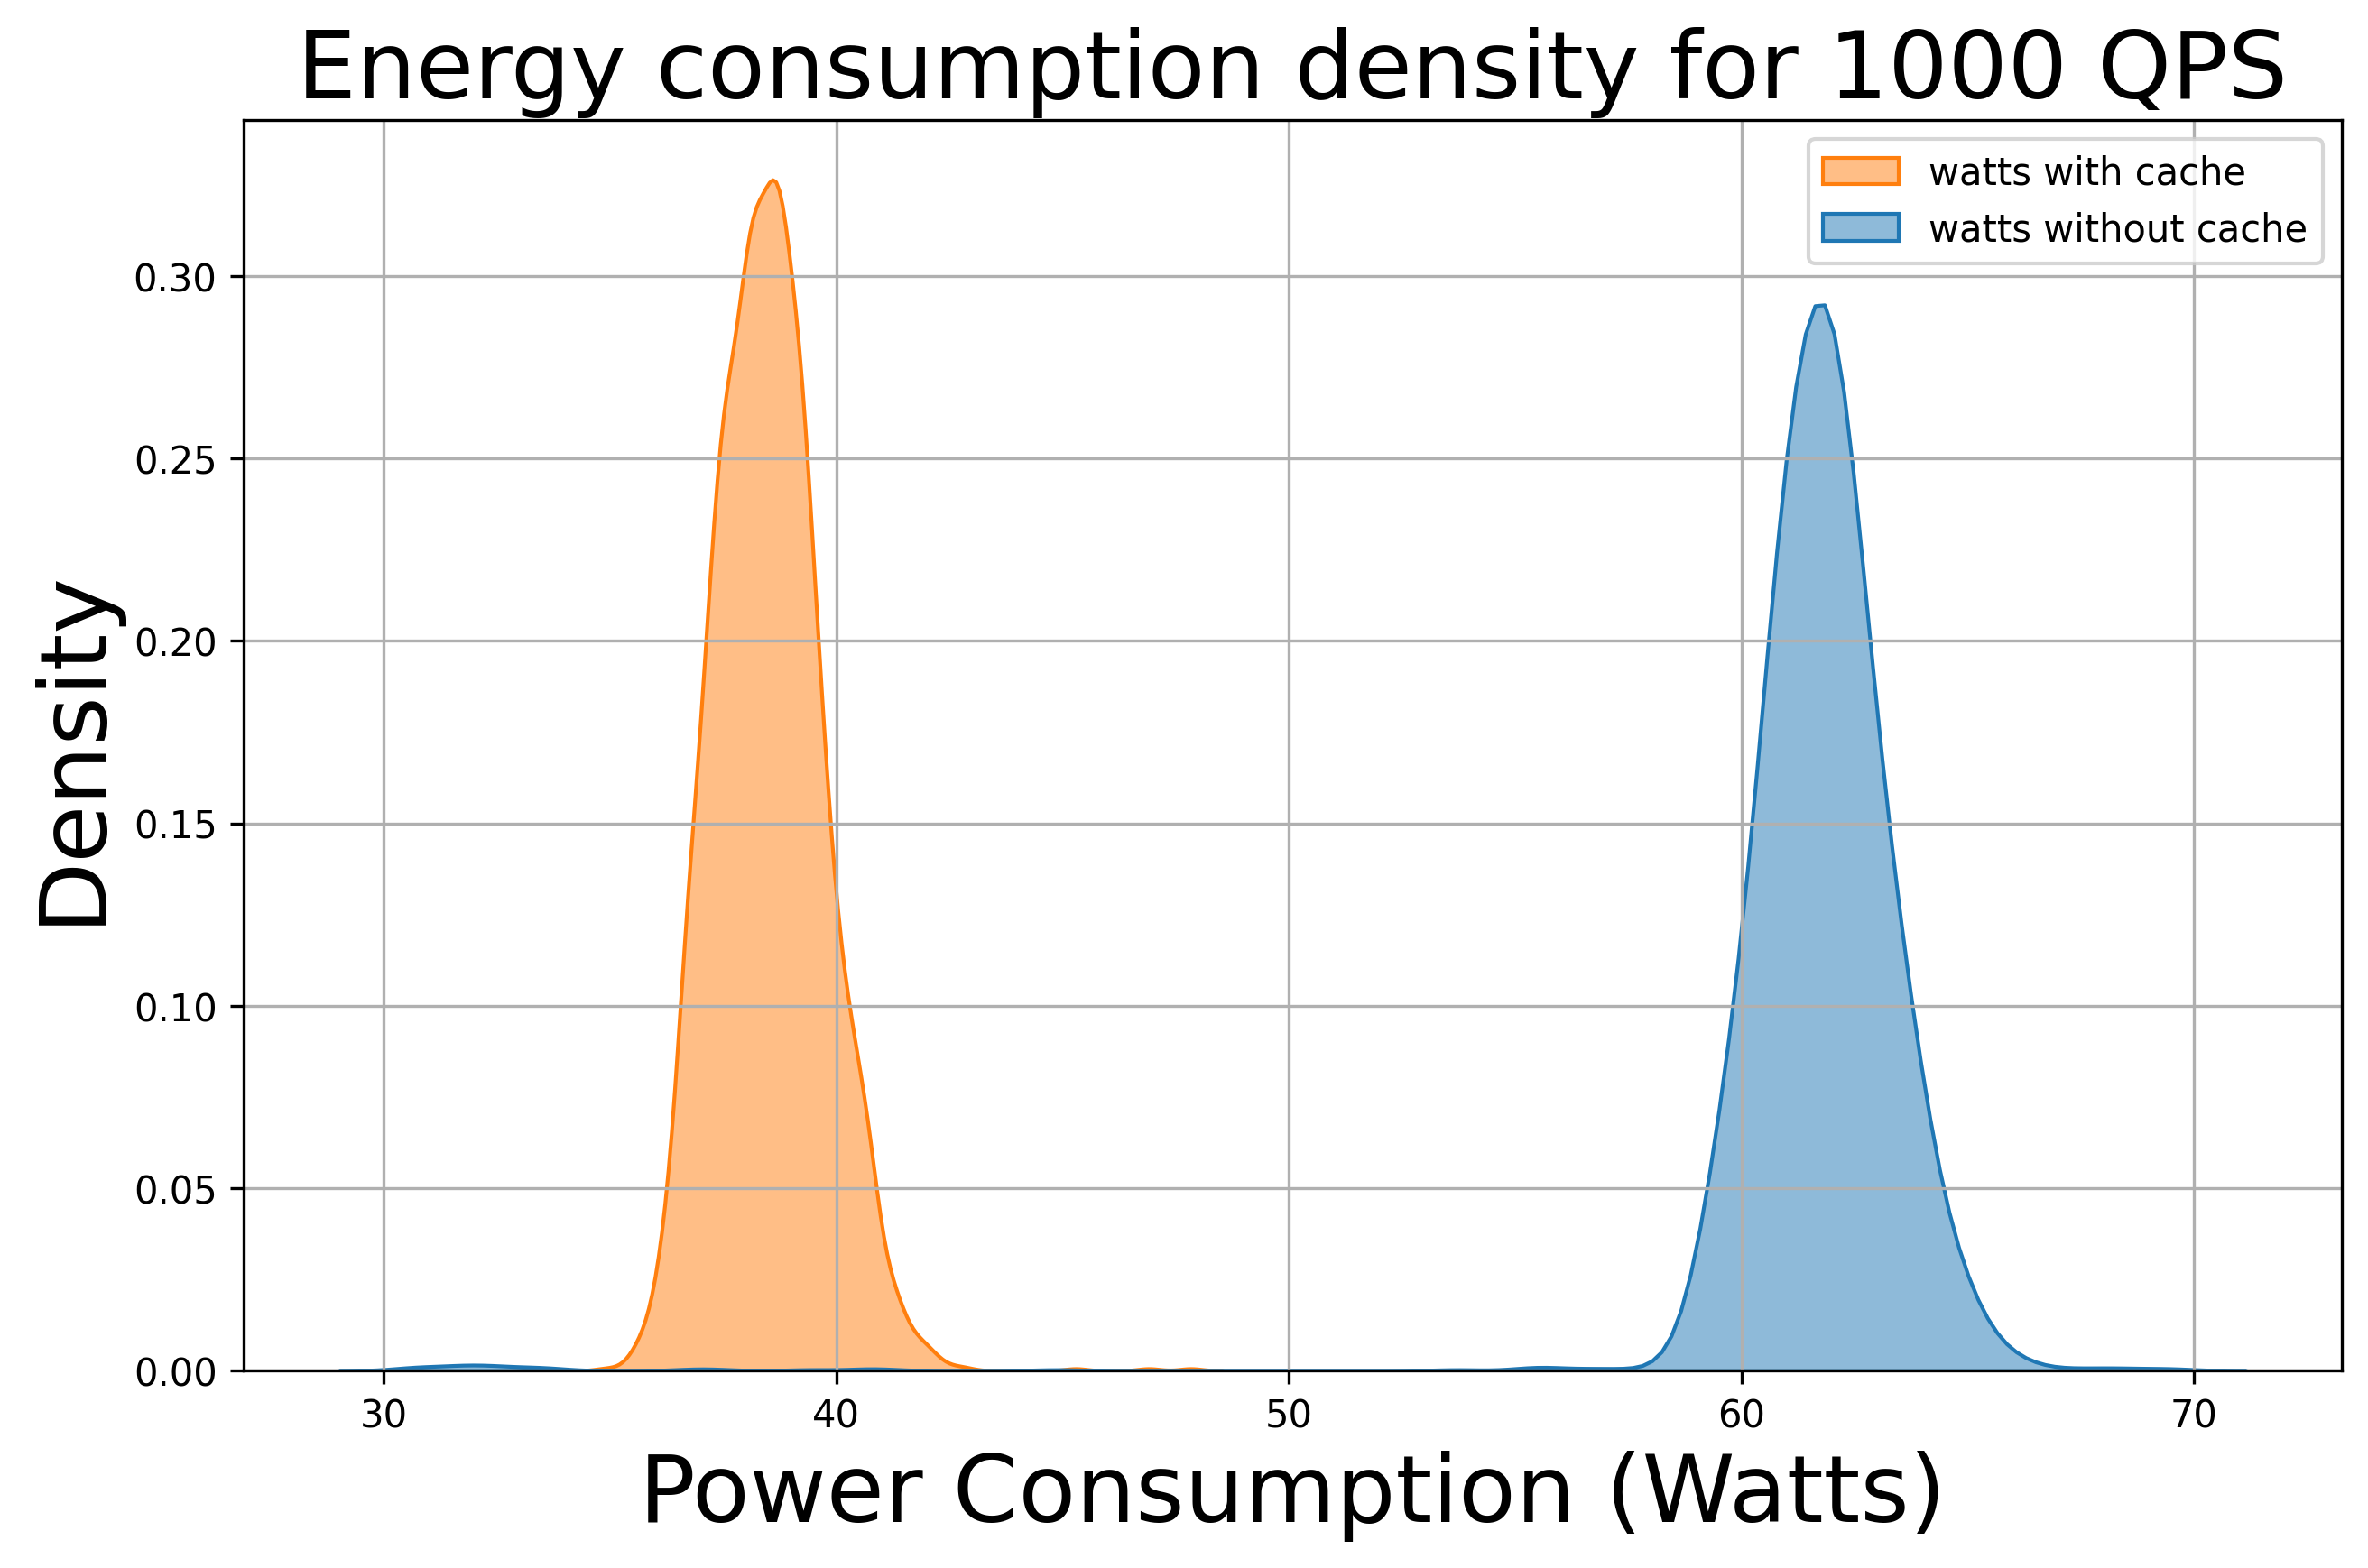
\includegraphics[width=\textwidth]{Graphs/consumption_density_qps_1000_udp.png}
		\end{minipage}
	\end{figure}
	
	Cela est réalisé à l'aide d'estimations de densité par noyau (*Kernel Density Estimations*).
	
	---
	\subsubsection{Différence entre cache et non-cache}
	
	La différence de consommation entre la résolution avec et sans cache est claire et nous pouvons modéliser cette différence. Le modèle n'est pas directement appliqué à la différence car les QPS dans les mesures ne sont pas les mêmes avec et sans cache. Ainsi, pour modéliser cette différence, nous commençons par modéliser les courbes avec et sans cache pour chaque protocole, puis nous faisons simplement la différence entre elles.
	
	\begin{figure}[H]
		\centering
		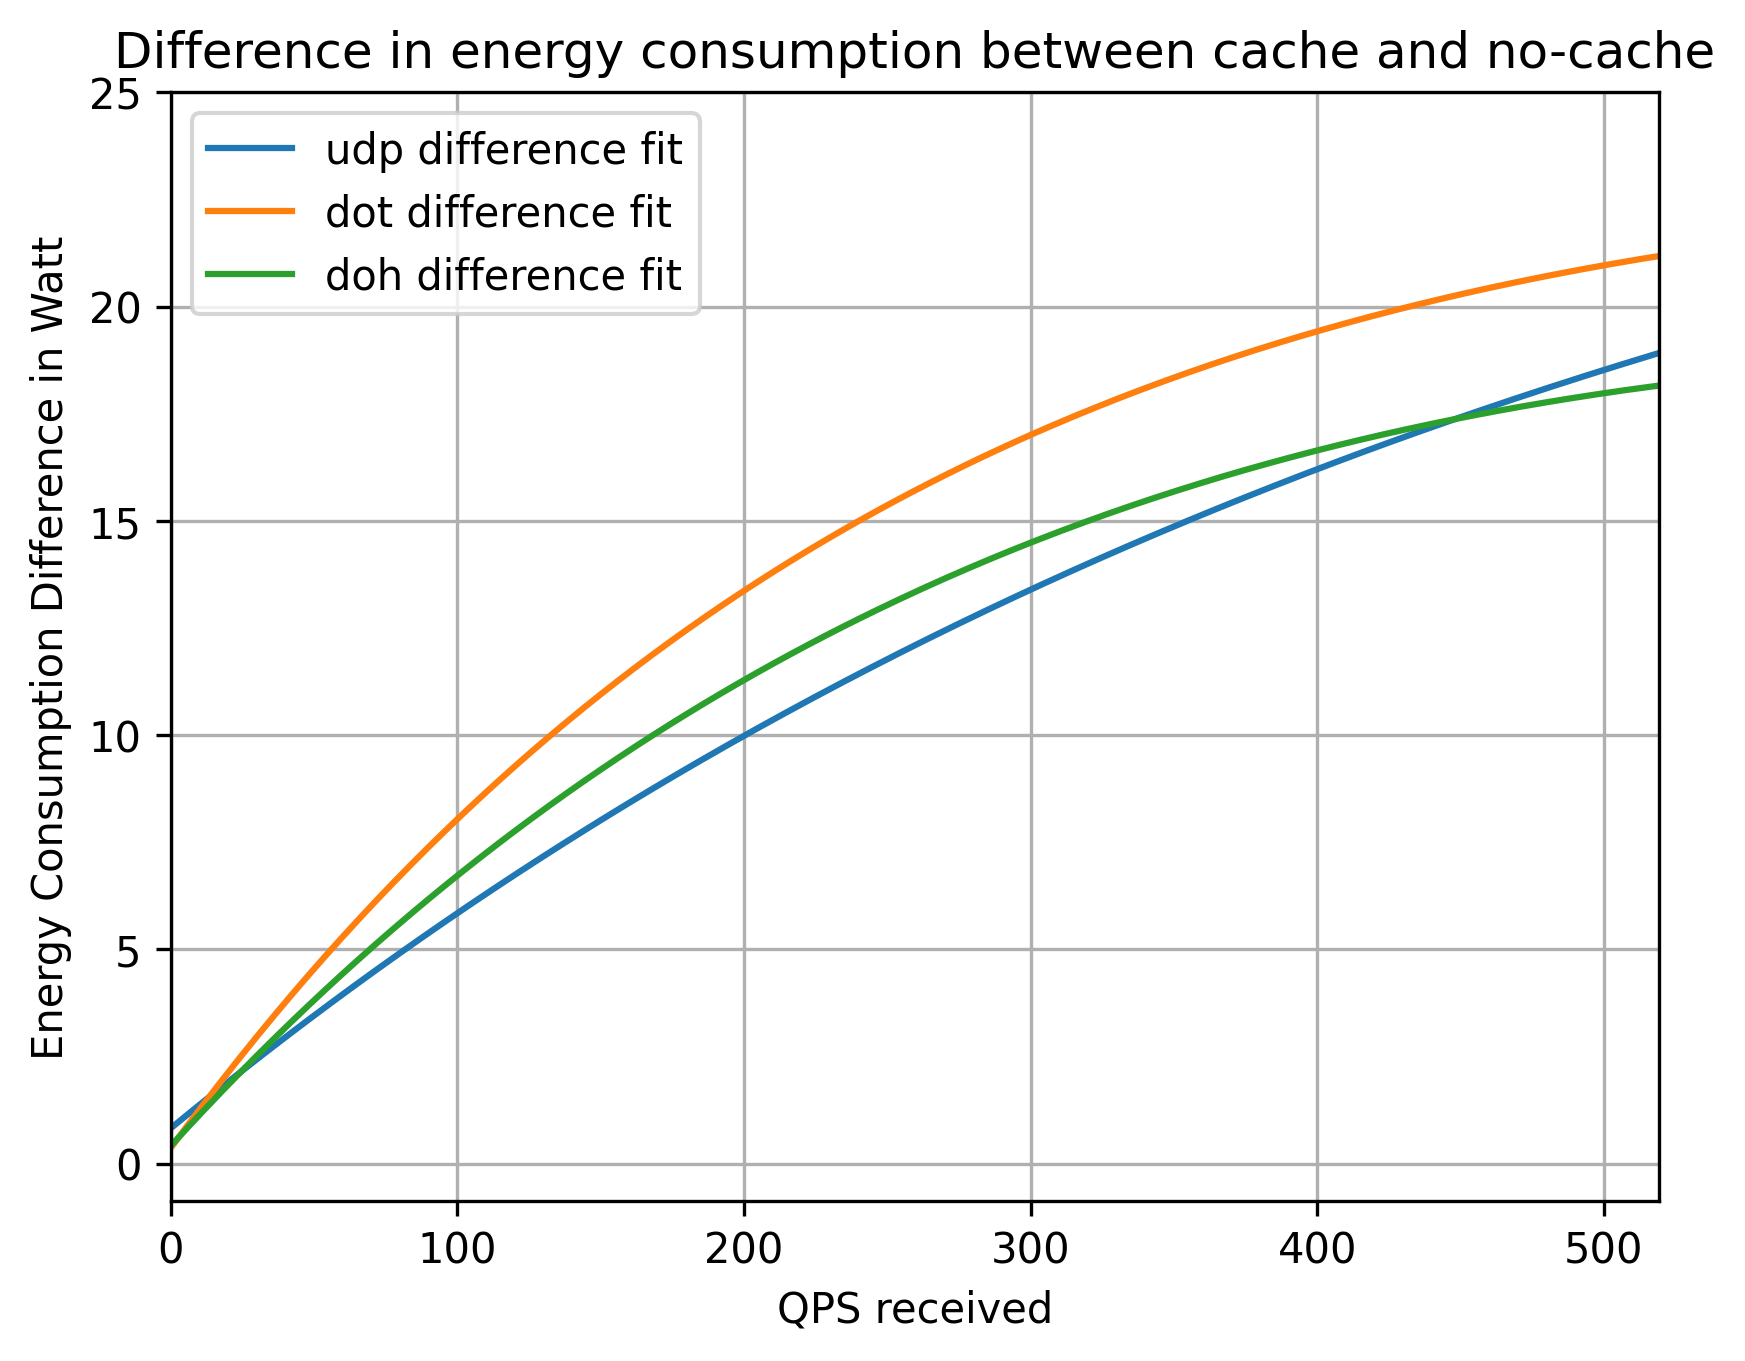
\includegraphics[width=0.9\textwidth]{Graphs/energy_consumption_difference.png}
		\caption{Différence de consommation entre les résolutions avec et sans cache}
		\label{fig:image3}
	\end{figure}
	
	La courbe a la forme d'une décroissance exponentielle car c'est ce que nous avons utilisé pour modéliser les consommations avec et sans cache.
	
	\subsubsection{Nouvelle méthodologie de mesure}
	
	Il y a certains problèmes avec les mesures. Pour les résoudre, la méthodologie doit être ajustée. Ces ajustements devraient résoudre les problèmes suivants :
	\begin{itemize}
		\item Le même ensemble de domaines pour les mesures avec et sans cache n'est pas utilisé.
		\item Nous ne pouvons pas vraiment savoir si le cache est vraiment utilisé ou non.
	\end{itemize}
	
	Les étapes pour ces ajustements sont :
	\begin{enumerate}
		\item Mesurer l'utilisation du cache pour différentes tailles d'ensembles de domaines.
		\item Sélectionner un ensemble de domaines qui sature le cache, mais où toutes les requêtes touchent le cache pour estimer la consommation énergétique du cache.
		\item Définir le TTL maximum du cache à 0 pour les mesures sans utilisation du cache et à 7 jours pour les mesures avec utilisation du cache.
	\end{enumerate}
	
	Cela permettra de mesurer avec précision la consommation de recherche dans le cache en fonction de sa taille et avec le même ensemble de domaines.
	
	\subsubsection{Modifications de la configuration}
	Entre chaque mesure, la configuration sera modifiée. Tout d'abord, le cache sera vidé, puis le TTL maximum du cache sera défini à 0 si les mesures se concentrent sur l'absence de cache, et à 7 jours s'il se concentre sur l'utilisation du cache.
	
	\subsubsection{Nouvelles métriques}
	Le cache sera surveillé à l'aide de 6 variables disponibles via \texttt{rndc}, un module utilisé pour visualiser les métriques de Bind9.
	
	Les nouvelles métriques sont :
	
	\begin{description}
		\item[Accès au cache] \hfill \\
		Le nombre total de requêtes DNS \textbf{servies directement depuis le cache}. \\
		Cela inclut les réponses positives (par exemple, les enregistrements A, AAAA, MX) qui ont été précédemment mises en cache. \\
		\textit{Unité : Compteur (entier non signé).}
		
		\item[Échecs de cache] \hfill \\
		Le nombre total de requêtes DNS \textbf{non servies depuis le cache}, nécessitant une résolution externe (par exemple, en interrogeant un serveur DNS autoritatif ou récursif). \\
		\textit{Unité : Compteur (entier non signé).}
		
		\item[Accès au cache (à partir des requêtes)] \hfill \\
		Le nombre de \textbf{réponses en cache} pour les requêtes entrantes. \\
		Contrairement aux \texttt{accès au cache}, cette métrique se concentre sur les \textbf{requêtes initiales} servies depuis le cache. \\
		\textit{Unité : Compteur (entier non signé).}
		
		\item[Échecs de cache (à partir des requêtes)] \hfill \\
		Le nombre de requêtes entrantes \textbf{non résolues par le cache}, nécessitant une résolution externe. \\
		Complémentaire aux \texttt{accès au cache (à partir des requêtes)} pour évaluer l'efficacité du cache sur les requêtes entrantes. \\
		\textit{Unité : Compteur (entier non signé).}
		
		\item[Mémoire de l'arbre de cache] \hfill \\
		Mémoire \textbf{utilisée par la structure arborescente du cache} (en octets). \\
		Représente la mémoire allouée pour organiser les entrées du cache dans une structure arborescente (optimisée pour des recherches rapides). \\
		\textit{Unité : Octets.}
		
		\item[Mémoire du tas de cache] \hfill \\
		Mémoire \textbf{utilisée par le tas du cache} (en octets). \\
		Représente la mémoire allouée dynamiquement pour les entrées du cache non organisées dans l'arbre. \\
		\textit{Unité : Octets.}

		\item[Entrées de cache supprimées en raison de l'épuisement de la mémoire] \hfill \\
		Le nombre d'\textbf{entrées de cache supprimées} en raison de \textbf{l'épuisement de la mémoire}. \\
		Indique que le cache a atteint sa limite de mémoire allouée (\texttt{max-cache-size}) et a dû supprimer des entrées pour libérer de l'espace. \\
		\textit{Unité : Compteur (entier non signé).} \\
		\textit{Note : Une valeur > 0 suggère que \texttt{max-cache-size} devrait être augmentée.}
		
		\item[Entrées de cache supprimées en raison de l'expiration du TTL] \hfill \\
		Le nombre d'\textbf{entrées de cache supprimées} car leur \textbf{TTL (*Time To Live*) a expiré}. \\
		Représente le nombre d'enregistrements DNS automatiquement supprimés du cache après avoir atteint leur durée de vie maximale. \\
		\textit{Unité : Compteur (entier non signé).}
	\end{description}

	\subsubsection{Étude de la distribution des types de requêtes et des TTLs}
		
	Une manière de visualiser l'utilisation du résolveur consiste à examiner chaque paquet envoyé et reçu par le résolveur. Sachant que Bind9 utilise UDP pour communiquer avec les DNS autoritatifs, l'examen des paquets UDP est idéal. Ces paquets incluent de nombreux types de requêtes que nous verrons juste en dessous. Ces nombres de requêtes sont divisés par le QPS résolu par le résolveur.
	
	Pour les mesures utilisant UDP, comme le résolveur utilise également UDP, pour éviter de mesurer les requêtes envoyées et reçues par le résolveur, nous déduisons 2 requêtes pour chaque résolution, ce qui correspond au modèle UDP.
	
	\begin{figure}[H]
		\centering
		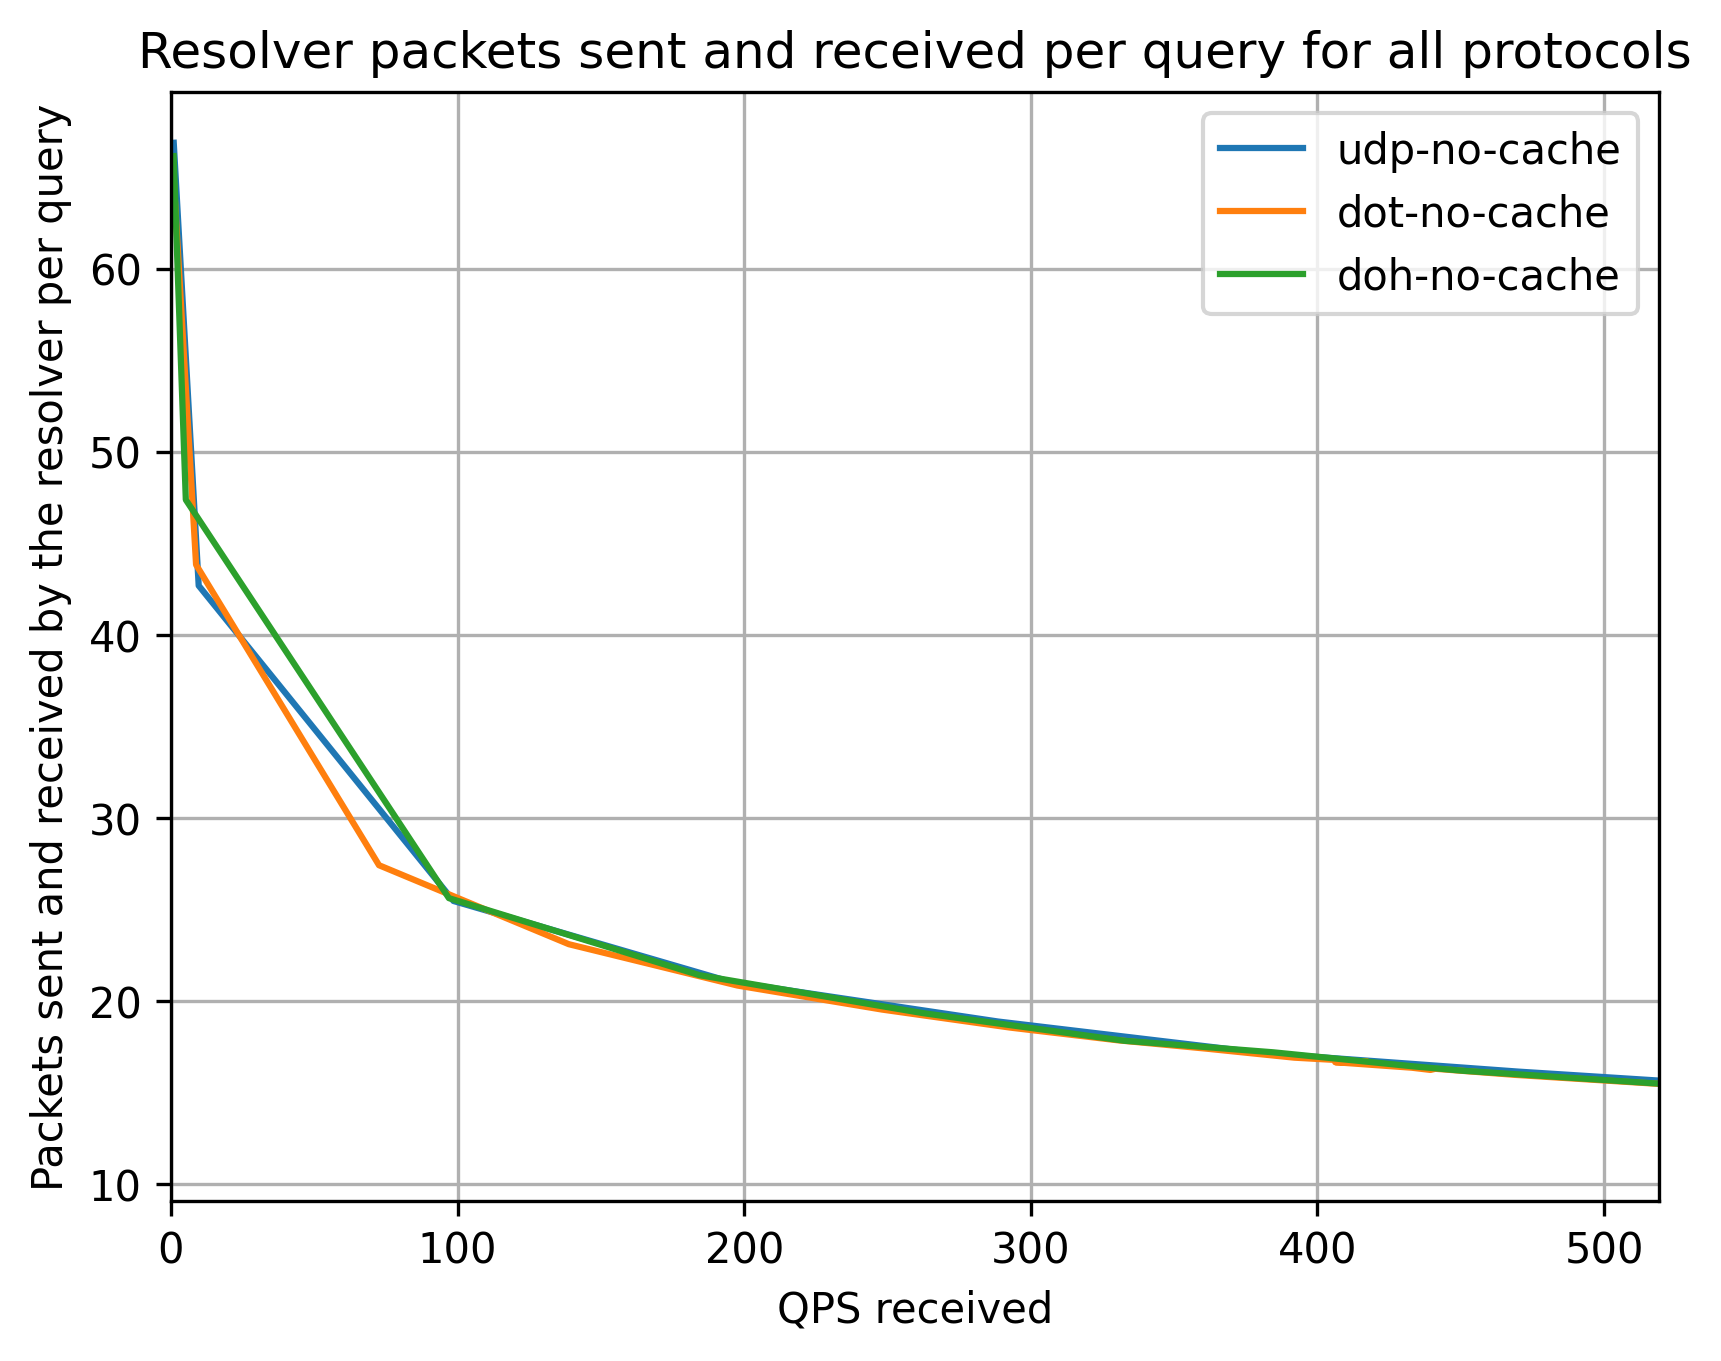
\includegraphics[width=0.9\textwidth]{Graphs/resolver_qps.png}
		\caption{Nombre de requêtes envoyées et reçues par le résolveur pour une résolution en fonction du QPS}
		\label{fig:image2}
	\end{figure}
	
	Le fait que cela suive une décroissance exponentielle est étrange et doit être étudié. La manière d'étudier cela consiste à examiner la distribution des types de requêtes pour chaque valeur afin de voir quels types de requêtes sont moins présents lorsque le QPS augmente.


	Toutes les requêtes récursives ne concernent pas des adresses IP : certaines sont des délégations vers un autre serveur autoritatif (NS), d'autres sont des alias vers un autre nom de domaine (CNAME). Il y a également des informations DNSSEC telles que RRSIG, DNSKEY, DS, etc.
	
	Ainsi, pour voir la distribution de ces requêtes, voici un exemple pour une configuration.
	
	\begin{figure}[H]
		\centering
		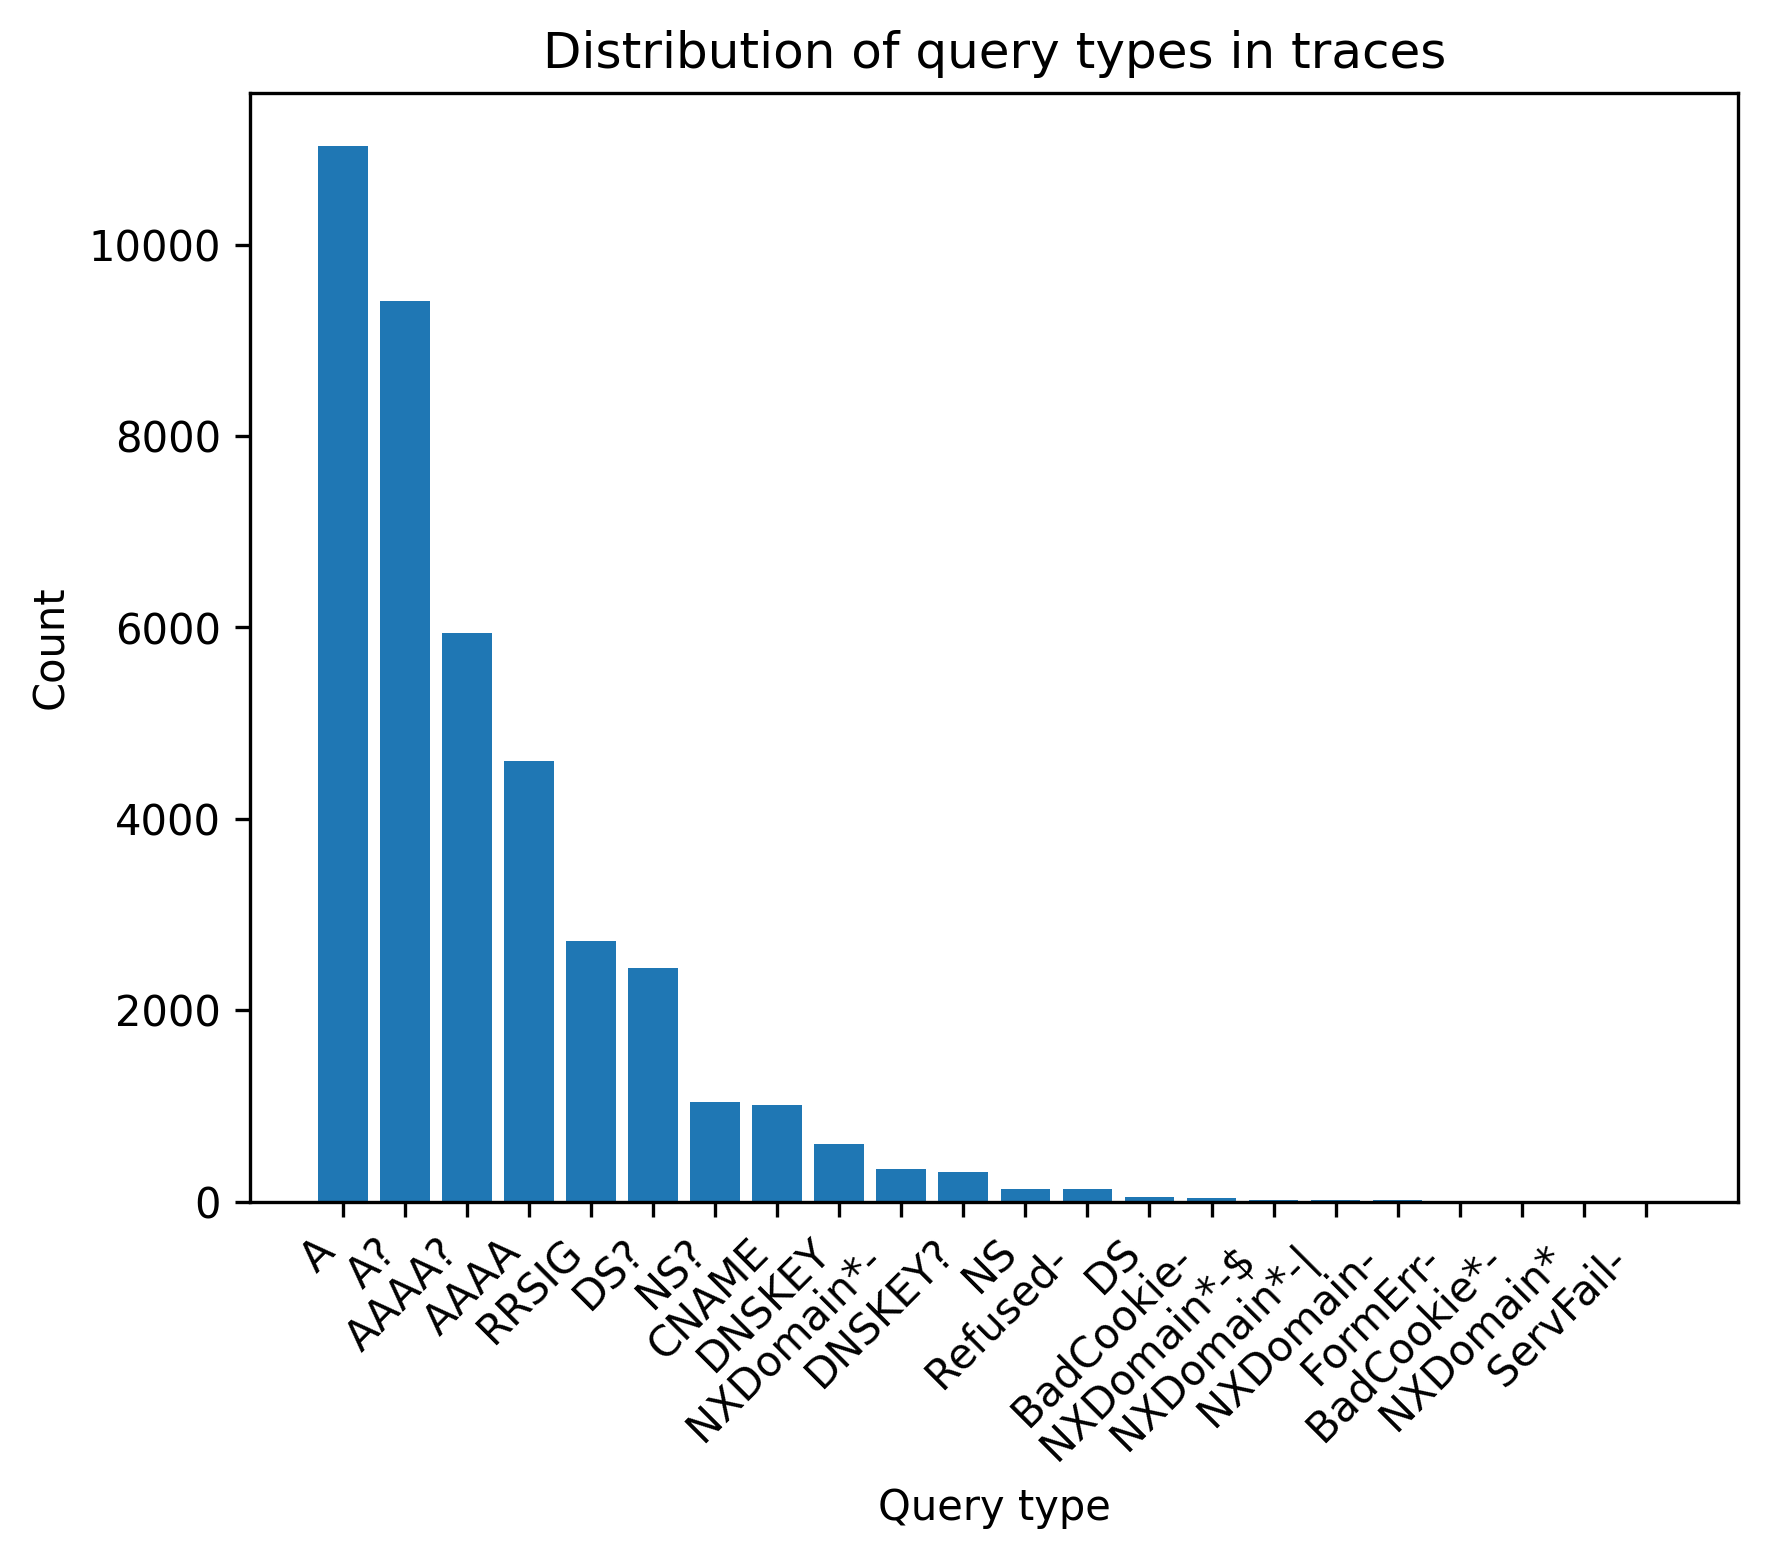
\includegraphics[width=0.9\textwidth]{Graphs/query_type_distribution.png}
		\caption{Distribution des types de requêtes pour les résolutions récursives}
		\label{fig:image4}
	\end{figure}
	
	La plupart sont de type IP, mais il y a une part non négligeable de DNSSEC, NS et CNAME.
	
	Le cache permet d'économiser beaucoup de consommation énergétique, mais les entrées du cache ont une durée limitée spécifiée par les serveurs DNS autoritatifs\footnote{Cela est dû au fait que l'adresse IP peut changer au fil du temps ; de plus, les DNS sont généralement utilisés comme une première couche de répartiteurs de charge}. Il s'agit du TTL (*Time To Live*), spécifié en secondes dans la zone pour chaque entrée sur laquelle le DNS a autorité. La distribution de ce TTL est intéressante à examiner.
	
	Tout d'abord, nous pouvons examiner des noms de domaine aléatoires. Le graphique de gauche montre la CDF (*Cumulative Distribution Function*) de 100 000 noms de domaine aléatoires issus d'un ensemble d'1 million de noms de domaine pour avoir une idée de cette distribution. Le graphique de droite montre la distribution des TTL pour les TLD (*Top Level Domains*, comme .fr, .com), au total 192 (le nombre exact n'est pas confirmé).
	
	\begin{figure}[H]
		\centering
		\begin{minipage}{0.45\textwidth}
			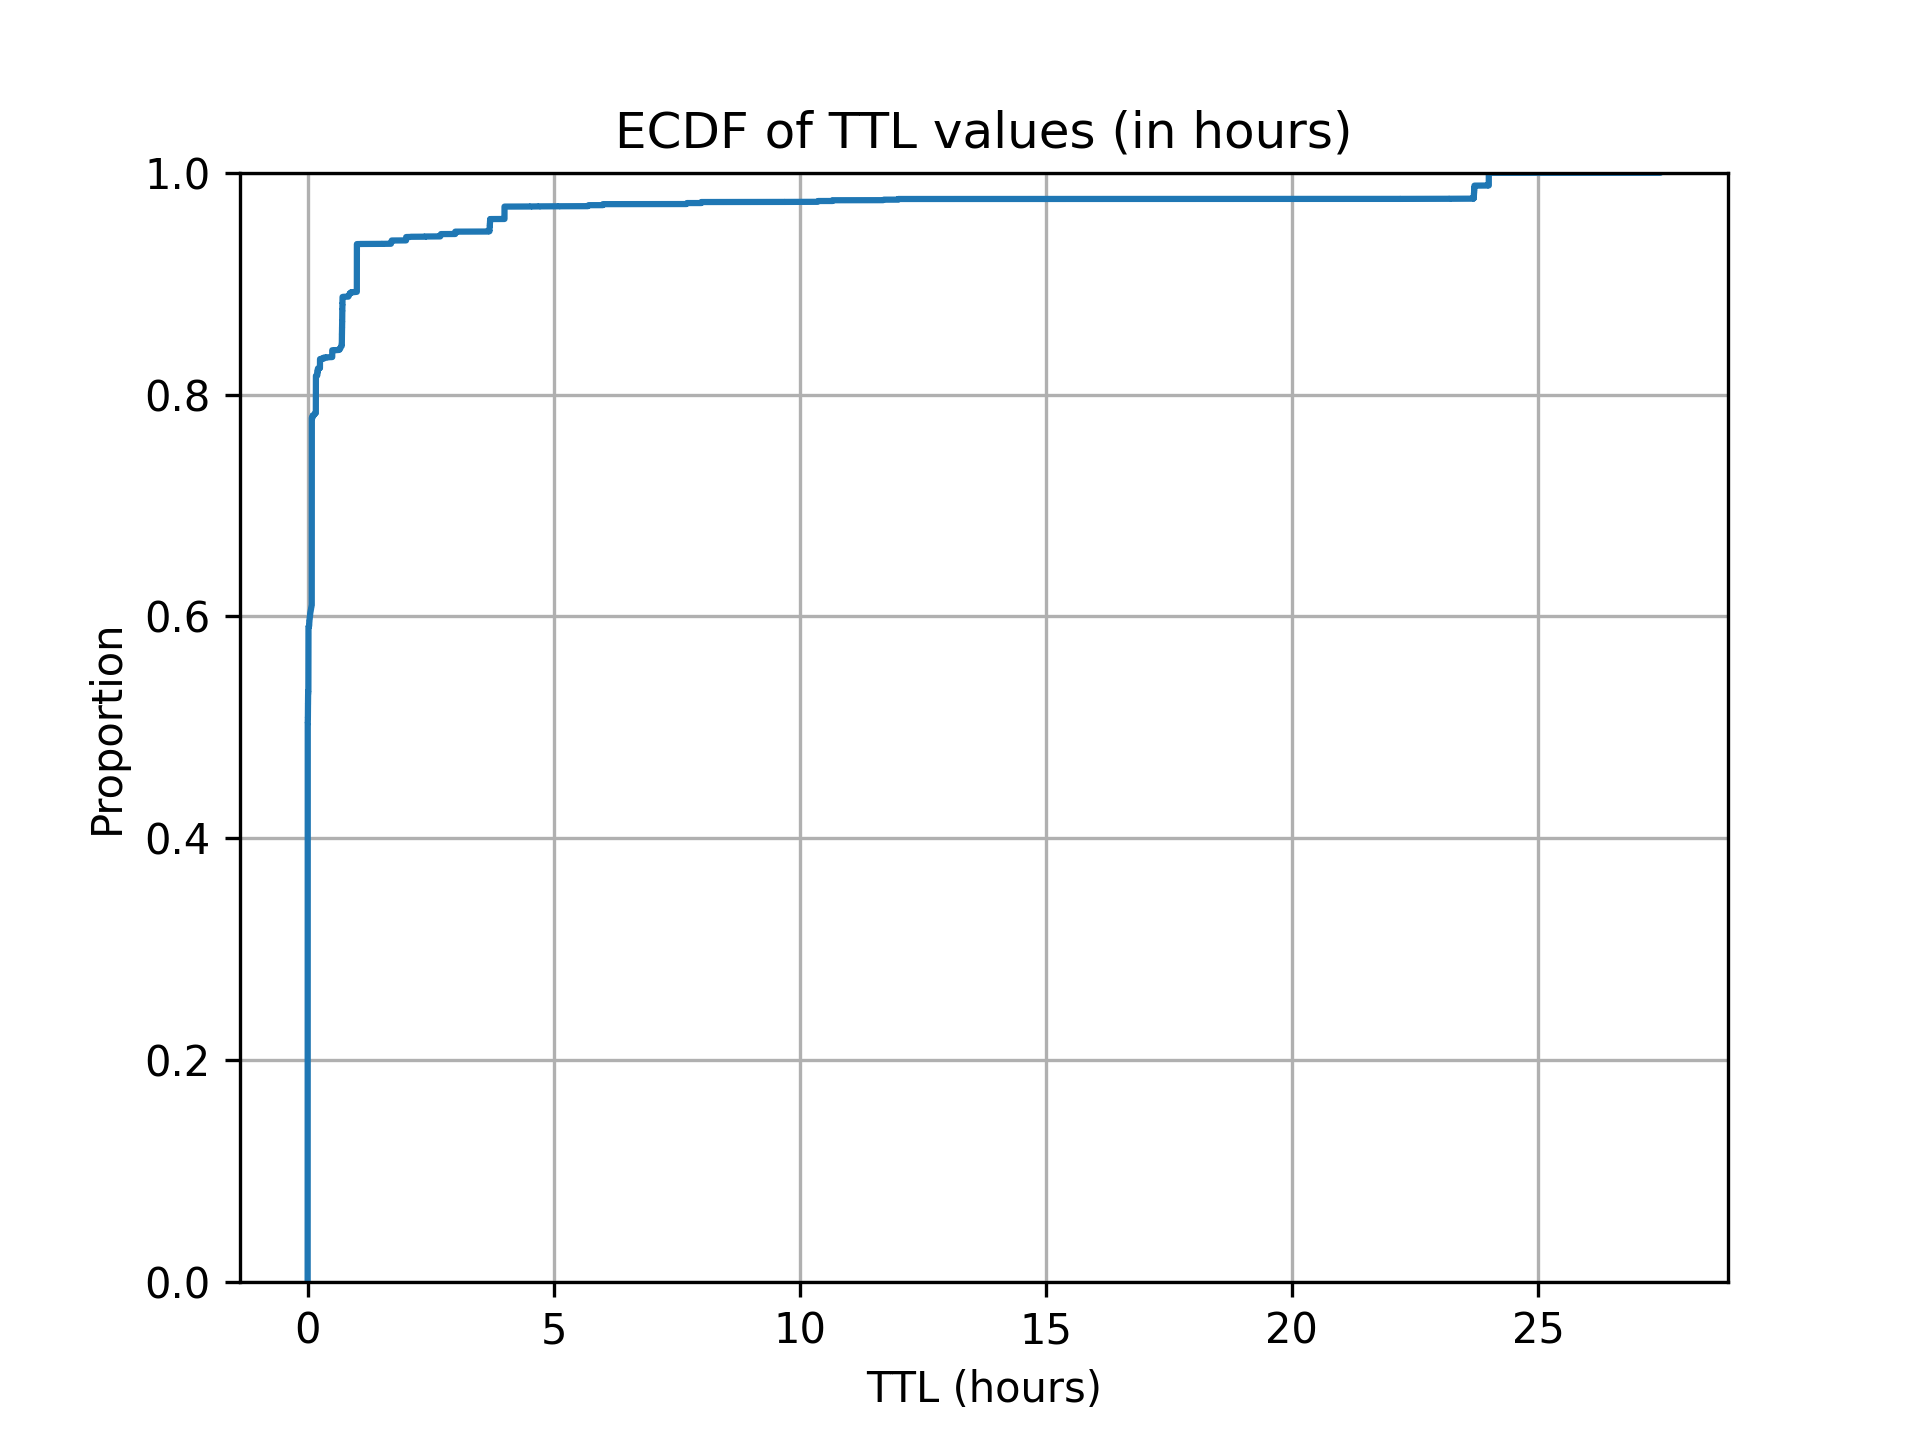
\includegraphics[width=\textwidth]{Graphs/ttl_ecdf.png}
		\end{minipage}
		\hfill
		\begin{minipage}{0.45\textwidth}
			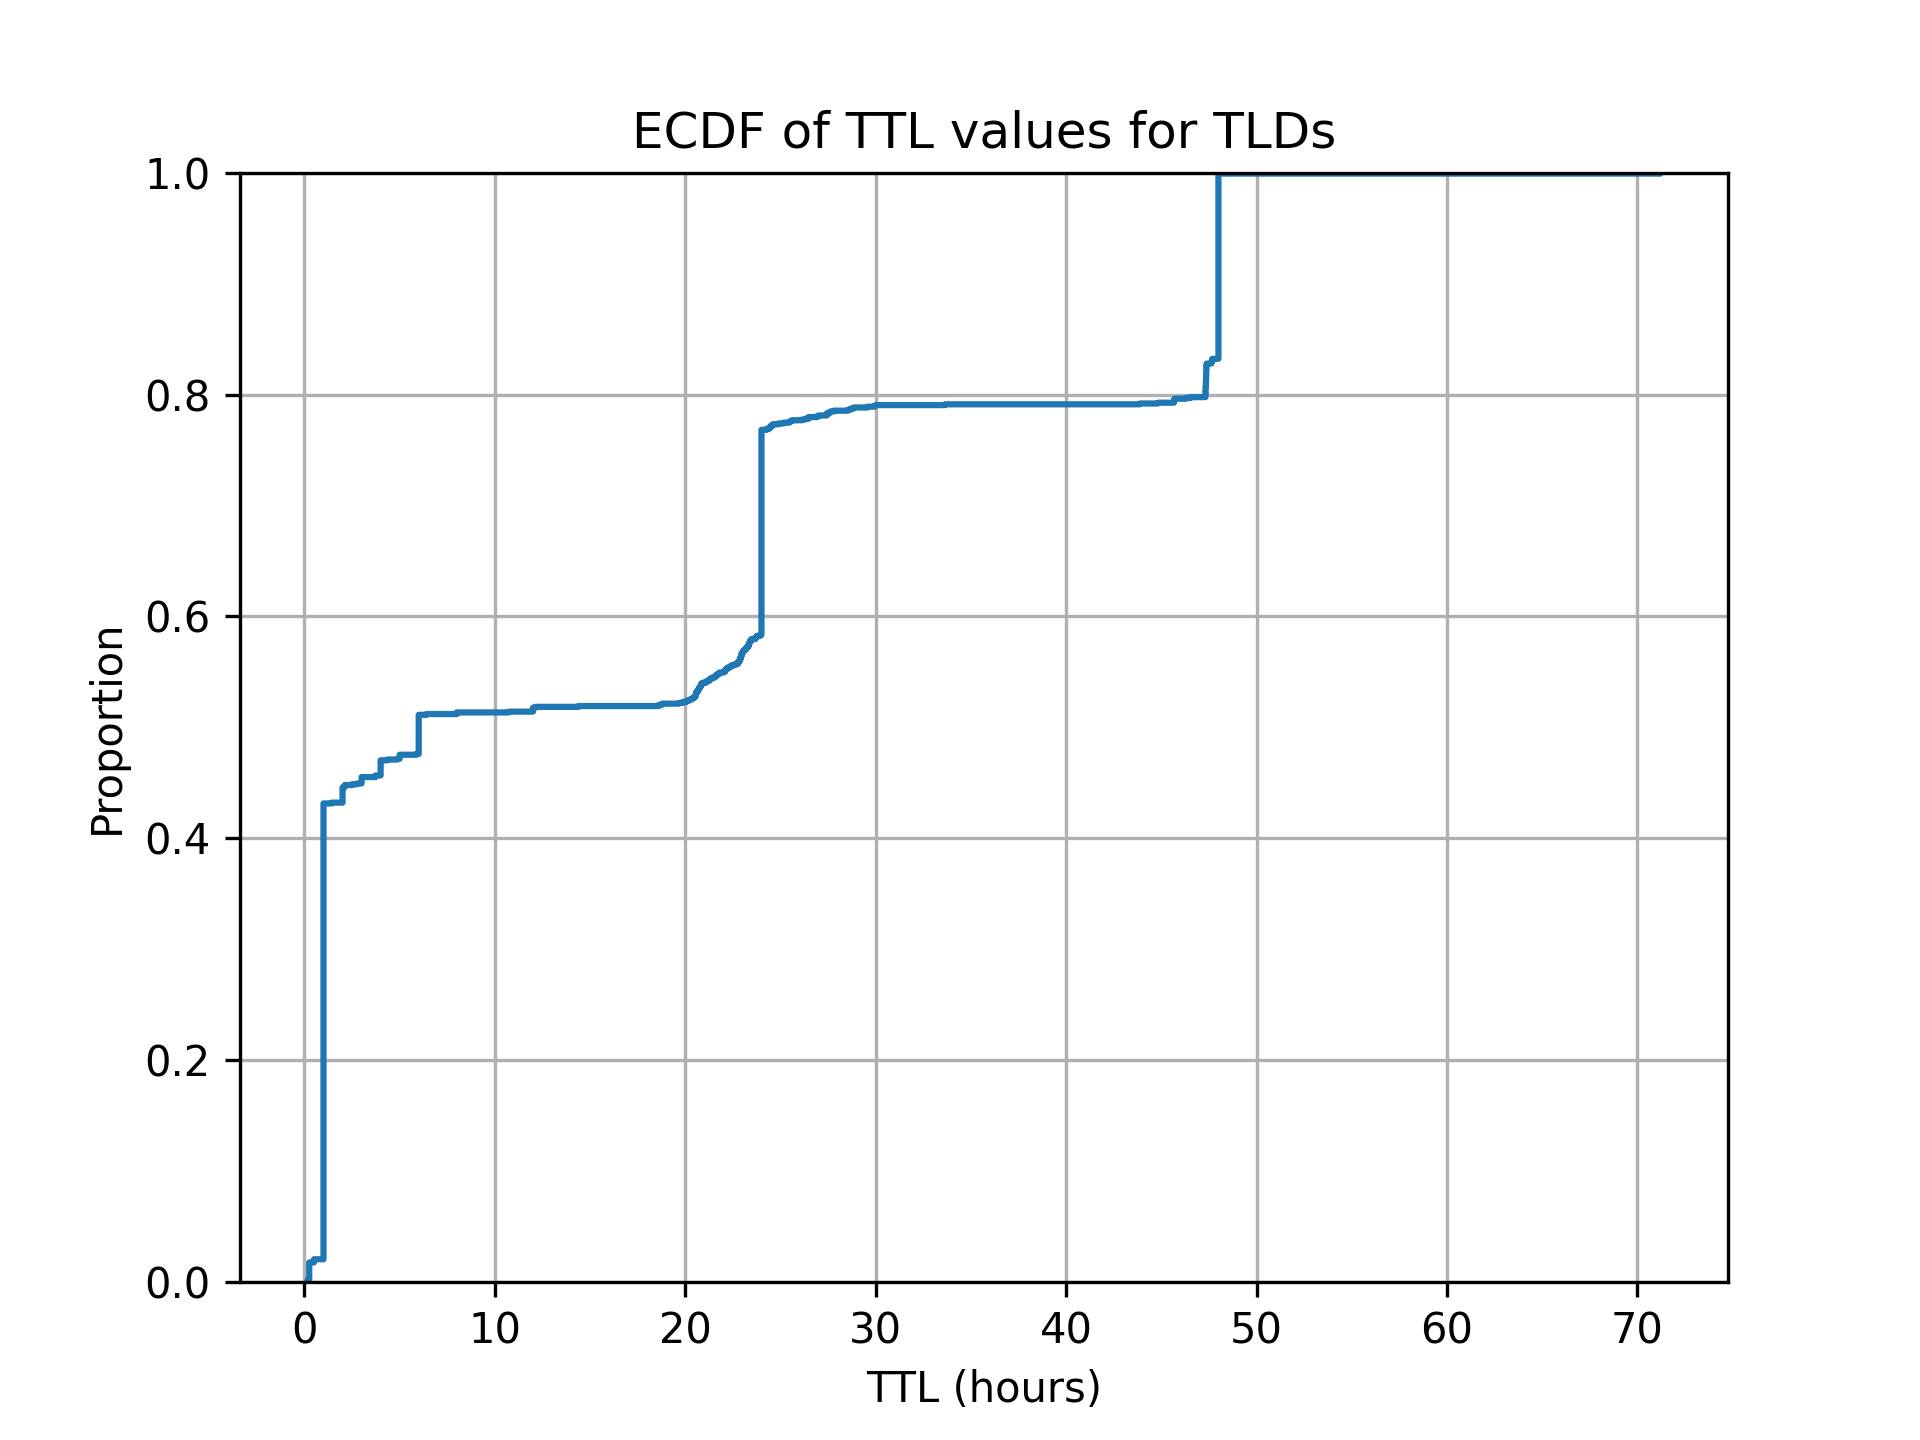
\includegraphics[width=\textwidth]{Graphs/tld_ttl_ecdf.png}
		\end{minipage}
	\end{figure}
	
	Pour les TLD, des pics peuvent être observés à 24h et 48h car ce sont des valeurs rondes.

	\subsubsection{Étude d'ablation}
	
	\subsubsection{Étude de la complexité algorithmique de Bind9}
	
	\subsection{Modélisation}
	
	Introduction des modèles et comparaison.

	\subsubsection{Prédiction de la consommation énergétique du DNS}
	
	À partir de toutes les métriques collectées lors des mesures, il est possible d'entraîner un modèle pour prédire avec précision la consommation énergétique du DNS. Le modèle qui donne les meilleurs résultats est un modèle de régression linéaire.
	
	\begin{figure}[H]
		\centering
		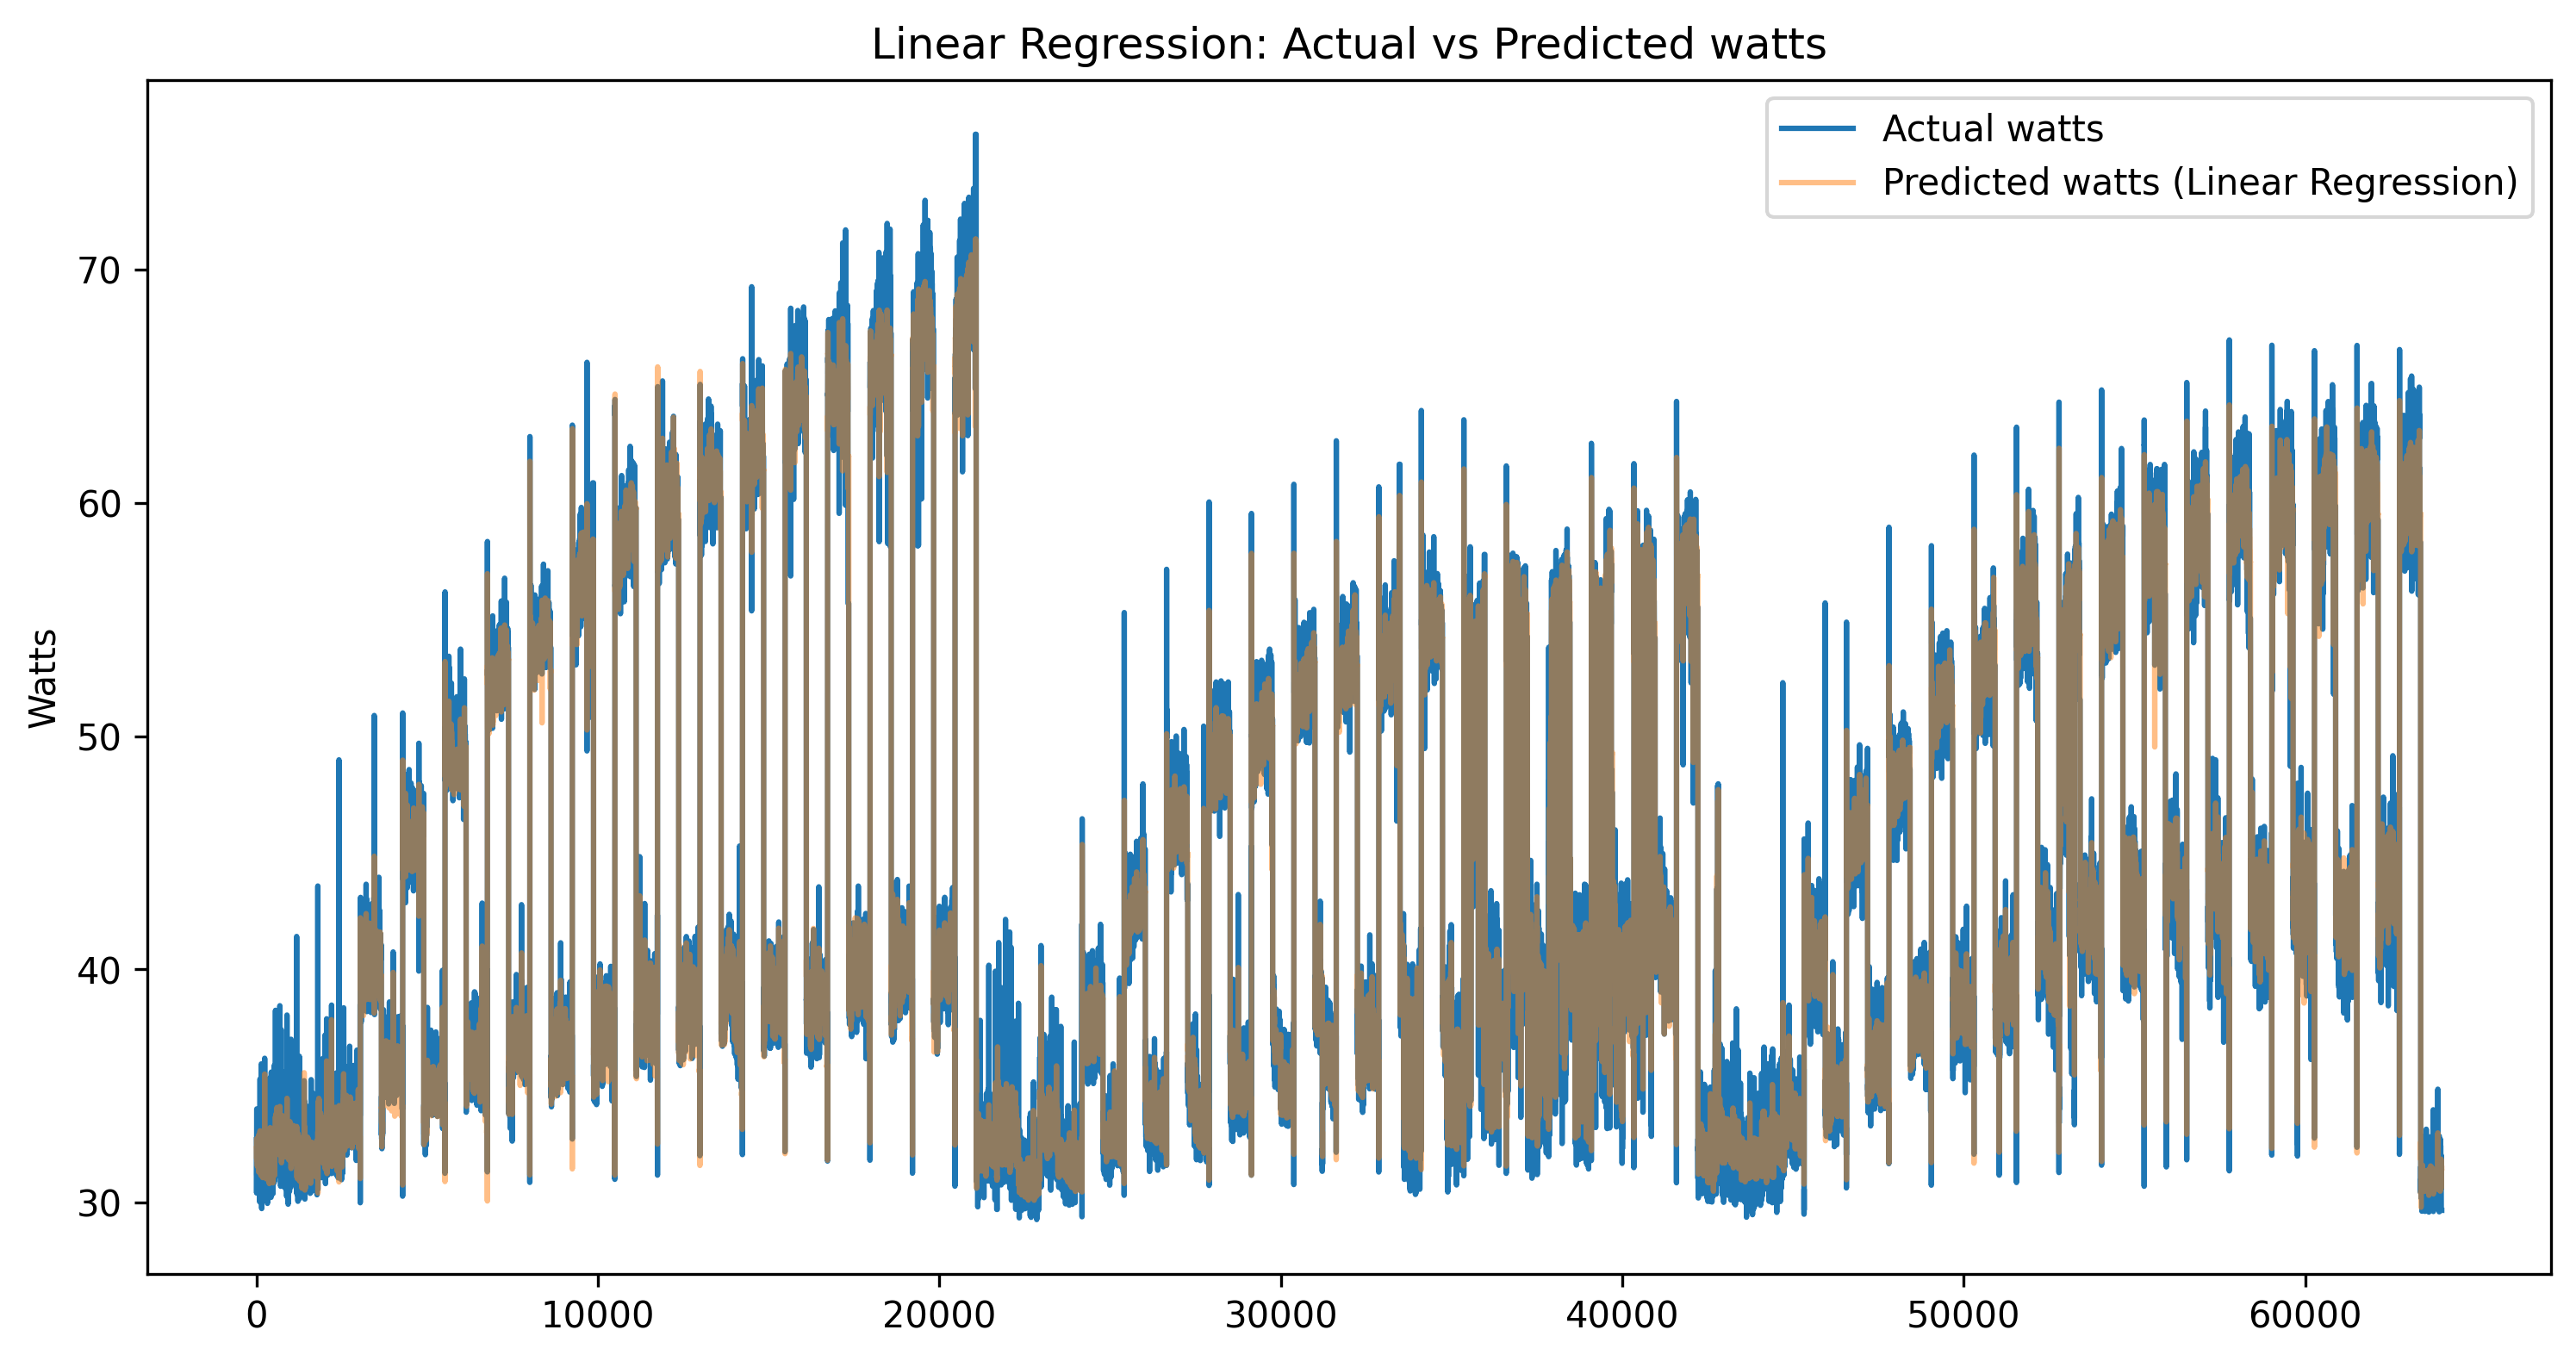
\includegraphics[width=0.9\textwidth]{Graphs/linear_regression_predictions.png}
		\caption{Estimation par régression linéaire et consommation énergétique réelle}
		\label{fig:image5}
	\end{figure}
	
	
	\subsubsection{Modèle de réseau de files d'attente}

	Une manière d'estimer la consommation d'un résolveur DNS consiste à comprendre les étapes d'une résolution et à estimer la consommation de chacune de ces étapes pour avoir une approche plus généraliste. Cela permettra d'estimer la consommation d'un résolveur indépendamment du matériel, de la charge et de la configuration de l'implémentation.

	Les réseaux de files d'attente sont parfaits pour ce type de décomposition, car ils peuvent représenter différents types de retards dus au temps d'attente ou au traitement.

	À partir de notre compréhension de Bind9, nous avons créé un modèle de réseau de files d'attente. Il se compose de plusieurs parties représentant les principales étapes de la résolution DNS, y compris la connexion. Ces étapes sont :
	\begin{itemize}
		\item Connexion TCP (si utilisation de DoT ou DoH)
		\item Poignée de main TCP (établissement de la connexion)
		\item Échange de certificats TLS
		\item Résolution récursive composée de :
		\begin{itemize}
			\item Threads de travail
			\item Requêtes DNS aux serveurs autoritatifs
		\end{itemize}
		\item Recherche dans le cache / insertion dans le cache
	\end{itemize}

	Chacune de ces étapes est modélisée par un modèle de file d'attente M/M/C, avec ses caractéristiques qui seront estimées à l'aide de mesures.

	Une étude d'ablation aide à différencier la latence et la consommation de chaque composant (principalement CPU et RAM) pour établir les caractéristiques. Les caractéristiques à estimer sont :
	\begin{itemize}
		\item $\rho$ : Charge
		\item $S$ : Temps de service
	\end{itemize}

	L'étude d'ablation consiste à effectuer plusieurs mesures, d'abord avec une configuration nécessitant le minimum d'étapes dans la résolution DNS, puis en ajoutant progressivement ces étapes pour avoir une vision claire de l'étape qui agit dans chaque mesure, en considérant que chaque étape est indépendante.

	La méthodologie de mesure correspondant à chaque étape est :
	\begin{itemize}
		\item Threads de travail : Mesurés avec des requêtes UDP où le nom de domaine est déjà dans le cache pour éviter la résolution récursive.
		\item Recherche dans le cache : Mesurée avec UDP avec différentes charges de cache (mémoire occupée par le cache).
		\item Requêtes DNS aux serveurs autoritatifs : Mesurées avec des requêtes UDP où le nom de domaine n'est pas dans le cache.
		\item Connexion TCP : Mesurée avec des requêtes TCP sans échange de clés ou de certificats.
		\item Poignée de main TCP : Mesurée
	\end{itemize}

	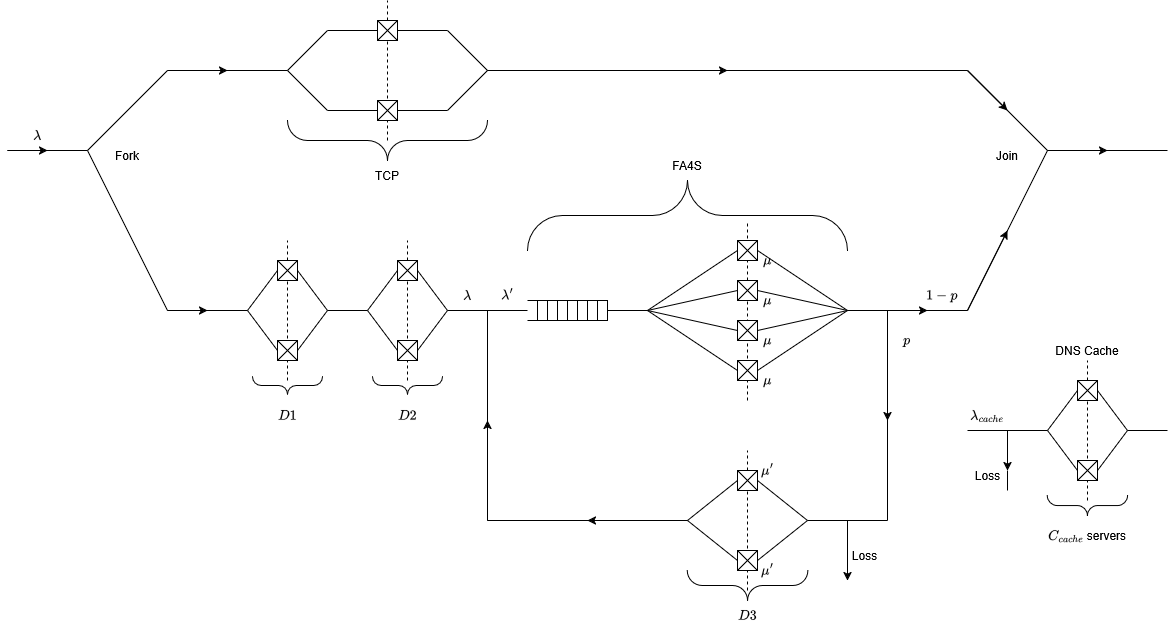
\includegraphics[width=0.9\textwidth]{diagrams_and_images/DNS_queue_model.png}

	Ce modèle est basé sur notre compréhension actuelle du \textbf{fonctionnement de Bind9}, et bien qu'il ne soit peut-être pas exhaustif, il fournit un \textbf{cadre fiable pour estimer la consommation énergétique}. Pour affiner sa précision, certains paramètres nécessiteront des mesures, suivies d'une analyse approfondie pour extraire et valider les données les plus pertinentes pour le modèle.

	---
	\subsubsection{Analyse de complexité algorithmique}

	Petite introduction / Pourquoi voulons-nous utiliser la complexité algorithmique pour ce problème ?

	Comment cela est-il fait ?

	Petite conclusion / Quel est le principal résultat de cela ?
	\cite{key}
	\chapter*{Conclusion}
	\addcontentsline{toc}{chapter}{Conclusion}

	\chapter*{Bibliographie}
	\addcontentsline{toc}{chapter}{Bibliographie}
	\nocite{*}
	\printbibliography{}

	\chapter*{Annexes}
	\addcontentsline{toc}{chapter}{Annexes}
	
	\section*{Détail des métriques collectées}
	\addcontentsline{toc}{section}{Détail des métriques collectées}
	

	\newpage


	\makeutbmbackcover{}
\end{document}
